\documentclass[portrait,final,a0paper,fontscale=0.277]{baposter}

\usepackage{calc}
\usepackage{graphicx}
\usepackage{amsmath}
\usepackage{amssymb}
\usepackage{relsize}
\usepackage{multirow}
\usepackage{rotating}
\usepackage{bm}
\usepackage{enumitem}
\usepackage{url}
\usepackage{booktabs}
 
\usepackage{tikz}
\usepackage{graphicx}
\usepackage{multicol}
\usepackage{algorithm}
\usepackage{algorithmic}
\usepackage{color, colortbl}
  %\floatname{algorithm}{algorithm}
  \renewcommand{\algorithmicrequire}{\textbf{Input:}}
  \renewcommand{\algorithmicensure}{\textbf{Output:}} 
%\usepackage{times}
%\usepackage{helvet}
%\usepackage{bookman}

\usepackage{anyfontsize}
\usepackage{palatino}
\usepackage{array}
\newcolumntype{C}[1]{>{\centering\let\newline\\\arraybackslash\hspace{0pt}}m{#1}}

\newcommand{\captionfont}{\footnotesize}

\graphicspath{{images/}{../images/}}
\usetikzlibrary{calc}


\newcommand{\Matrix}[1]{\begin{bmatrix} #1 \end{bmatrix}}
\newcommand{\Vector}[1]{\begin{pmatrix} #1 \end{pmatrix}}

\newcommand*{\norm}[1]{\mathopen\| #1 \mathclose\|}% use instead of $\|x\|$
\newcommand*{\abs}[1]{\mathopen| #1 \mathclose|}% use instead of $\|x\|$
\newcommand*{\normLR}[1]{\left\| #1 \right\|}% use instead of $\|x\|$

\newcommand*{\SET}[1]  {\ensuremath{\mathcal{#1}}}
\newcommand*{\FUN}[1]  {\ensuremath{\mathcal{#1}}}
\newcommand*{\MAT}[1]  {\ensuremath{\boldsymbol{#1}}}
\newcommand*{\VEC}[1]  {\ensuremath{\boldsymbol{#1}}}
\newcommand*{\CONST}[1]{\ensuremath{\mathit{#1}}}

\DeclareMathOperator*{\argmax}{arg\,max}
\DeclareMathOperator*{\diag}{diag}
\DeclareMathOperator*{\argmin}{arg\,min}
\DeclareMathOperator*{\vectorize}{vec}
\DeclareMathOperator*{\reshape}{reshape}

%\font\dsfnt=dsrom12

\newcommand{\SNN}{\ensuremath{\mathbb N}}
\newcommand{\SRR}{\ensuremath{\mathbb R}}
\newcommand{\SZZ}{\ensuremath{\mathbb Z}}
%-----------------------------------------------------------------------------
% Matrices of the shape model
\renewcommand{\a}{\VEC\alpha}
\renewcommand{\v}{\VEC v}
\renewcommand{\l}{\VEC l}
\newcommand*{\m}{\VEC{\mu}}
\newcommand*{\M}{\MAT{M}}
\renewcommand*{\P}{\MAT{\Pi}}

%\newcommand{\J}{\SET J}
\newcommand{\J}{\SET{P}}
\newcommand{\Active}{\mathcal{A}}
\newcommand{\Selection}{\mathbf{S}}
\newcommand{\AllSelections}{\mathfrak{S}}
\newcommand{\Params}{\VEC\Theta}

%%%%%%%%%%%%%%%%%%%%%%%%%%%%%%%%%%%%%%%%%%%%%%%%%%%%%%%%%%%%%%%%%%%%%%%%%%%%%%%%
%%%% Some math symbols used in the text
%%%%%%%%%%%%%%%%%%%%%%%%%%%%%%%%%%%%%%%%%%%%%%%%%%%%%%%%%%%%%%%%%%%%%%%%%%%%%%%%

%%%%%%%%%%%%%%%%%%%%%%%%%%%%%%%%%%%%%%%%%%%%%%%%%%%%%%%%%%%%%%%%%%%%%%%%%%%%%%%%
% Multicol Settings
%%%%%%%%%%%%%%%%%%%%%%%%%%%%%%%%%%%%%%%%%%%%%%%%%%%%%%%%%%%%%%%%%%%%%%%%%%%%%%%%
\setlength{\columnsep}{1.5em}
\setlength{\columnseprule}{0mm}

%%%%%%%%%%%%%%%%%%%%%%%%%%%%%%%%%%%%%%%%%%%%%%%%%%%%%%%%%%%%%%%%%%%%%%%%%%%%%%%%
% Save space in lists. Use this after the opening of the list
%%%%%%%%%%%%%%%%%%%%%%%%%%%%%%%%%%%%%%%%%%%%%%%%%%%%%%%%%%%%%%%%%%%%%%%%%%%%%%%%
\newcommand{\compresslist}{%
\setlength{\itemsep}{1pt}%
\setlength{\parskip}{0pt}%
\setlength{\parsep}{0pt}%
}

%%%%%%%%%%%%%%%%%%%%%%%%%%%%%%%%%%%%%%%%%%%%%%%%%%%%%%%%%%%%%%%%%%%%%%%%%%%%%%
%%% Begin of Document
%%%%%%%%%%%%%%%%%%%%%%%%%%%%%%%%%%%%%%%%%%%%%%%%%%%%%%%%%%%%%%%%%%%%%%%%%%%%%%
\usetikzlibrary{shapes.geometric}
\makeatletter
% the contents of \squarecorner were mostly stolen from pgfmoduleshapes.code.tex
\def\squarecorner#1{
    % Calculate x
    %
    % First, is width < minimum width?
    \pgf@x=\the\wd\pgfnodeparttextbox%
    \pgfmathsetlength\pgf@xc{\pgfkeysvalueof{/pgf/inner xsep}}%
    \advance\pgf@x by 2\pgf@xc%
    \pgfmathsetlength\pgf@xb{\pgfkeysvalueof{/pgf/minimum width}}%
    \ifdim\pgf@x<\pgf@xb%
        % yes, too small. Enlarge...
        \pgf@x=\pgf@xb%
    \fi%
    % Calculate y
    %
    % First, is height+depth < minimum height?
    \pgf@y=\ht\pgfnodeparttextbox%
    \advance\pgf@y by\dp\pgfnodeparttextbox%
    \pgfmathsetlength\pgf@yc{\pgfkeysvalueof{/pgf/inner ysep}}%
    \advance\pgf@y by 2\pgf@yc%
    \pgfmathsetlength\pgf@yb{\pgfkeysvalueof{/pgf/minimum height}}%
    \ifdim\pgf@y<\pgf@yb%
        % yes, too small. Enlarge...
        \pgf@y=\pgf@yb%
    \fi%
    %
    % this \ifdim is the actual part that makes the node dimensions square.
    \ifdim\pgf@x<\pgf@y%
        \pgf@x=\pgf@y%
    \else
        \pgf@y=\pgf@x%
    \fi
    %
    % Now, calculate right border: .5\wd\pgfnodeparttextbox + .5 \pgf@x + #1outer sep
    \pgf@x=#1.5\pgf@x%
    \advance\pgf@x by.5\wd\pgfnodeparttextbox%
    \pgfmathsetlength\pgf@xa{\pgfkeysvalueof{/pgf/outer xsep}}%
    \advance\pgf@x by#1\pgf@xa%
    % Now, calculate upper border: .5\ht-.5\dp + .5 \pgf@y + #1outer sep
    \pgf@y=#1.5\pgf@y%
    \advance\pgf@y by-.5\dp\pgfnodeparttextbox%
    \advance\pgf@y by.5\ht\pgfnodeparttextbox%
    \pgfmathsetlength\pgf@ya{\pgfkeysvalueof{/pgf/outer ysep}}%
    \advance\pgf@y by#1\pgf@ya%
}
\makeatother

\pgfdeclareshape{square}{
    \savedanchor\northeast{\squarecorner{}}
    \savedanchor\southwest{\squarecorner{-}}

    \foreach \x in {east,west} \foreach \y in {north,mid,base,south} {
        \inheritanchor[from=rectangle]{\y\space\x}
    }
    \foreach \x in {east,west,north,mid,base,south,center,text} {
        \inheritanchor[from=rectangle]{\x}
    }
    \inheritanchorborder[from=rectangle]
    \inheritbackgroundpath[from=rectangle]
}
\begin{document}

%%%%%%%%%%%%%%%%%%%%%%%%%%%%%%%%%%%%%%%%%%%%%%%%%%%%%%%%%%%%%%%%%%%%%%%%%%%%%%
%%% Here starts the poster
%%%---------------------------------------------------------------------------
%%% Format it to your taste with the options
%%%%%%%%%%%%%%%%%%%%%%%%%%%%%%%%%%%%%%%%%%%%%%%%%%%%%%%%%%%%%%%%%%%%%%%%%%%%%%
% Define some colors

\definecolor{lightorange}{rgb}{0.9,0.4,0}
\definecolor{lightestorange}{rgb}{1,0.8,0.5}
\definecolor{darkorange}{rgb}{0.4,0.2,0}
\definecolor{ch2}{rgb}{0.5,0.5,0.5}
\definecolor{blanco}{rgb}{1,1,1}
\definecolor{darkblue}{rgb}{0.0,0.0,0.75}

\hyphenation{resolution occlusions}
%%
\begin{poster}%
  % Poster Options
  {
  % Show grid to help with alignment
  grid=false,
  % Column 
  colspacing=1em,
  columns=6,
  % Color style
  bgColorOne=white,
  bgColorTwo=white,
  borderColor=black,
  headerColorOne=darkblue,
  headerColorTwo=ch2,
  headerFontColor=white,
  boxColorOne=blanco,
  boxColorTwo=blanco,
  % Format of textbox
  textborder=faded,
  % Format of text header
  eyecatcher=true,
  headerborder=closed,
  headerheight=0.1\textheight,
%   textfont={\noindent \bf},  
  textfont=\sc,% An example of changing the text font
  headershape=roundedright,
  headershade=shadelr,
  headerfont=\Large\bf\textsc, %Sans Serif
  textfont={\setlength{\parindent}{1.5em}},
  boxshade=plain,
%  background=shade-tb,
  background=plain,
  linewidth=2pt
  }
  % Eye Catcher
  {} 
  % Title
  {\bf\textsc{Two State Totalistic Freezing Cellular Automata}\vspace{0.5em}}
  % Authors diego.maldonado@univ-orleans.fr
  {\textsc{\small \{diego.maldonado, pedro.montealegre and nicolas.ollinger \}@univ-orleans.fr\\ eric.chacc@uai.cl}}
  % University logo
  {% The makebox allows the title to flow into the logo, this is a hack because of the L shaped logo.
    
\includegraphics[height=6em]{img/lifo}
  }

%%%%%%%%%%%%%%%%%%%%%%%%%%%%%%%%%%%%%%%%%%%%%%%%%%%%%%%%%%%%%%%%%%%%%%%%%%%%%%
%%% Now define the boxes that make up the poster
%%%---------------------------------------------------------------------------
%%% Each box has a name and can be placed absolutely or relatively.
%%% The only inconvenience is that you can only specify a relative position 
%%% towards an already declared box. So if you have a box attached to the 
%%% bottom, one to the top and a third one which should be in between, you 
%%% have to specify the top and bottom boxes before you specify the middle 
%%% box.
%%%%%%%%%%%%%%%%%%%%%%%%%%%%%%%%%%%%%%%%%%%%%%%%%%%%%%%%%%%%%%%%%%%%%%%%%%%%%%
    %
    % A coloured circle useful as a bullet with an adjustably strong filling
    \newcommand{\colouredcircle}{%
      \tikz{\useasboundingbox (-0.2em,-0.32em) rectangle(0.2em,0.32em); \draw[draw=black,fill=lightblue,line width=0.03em] (0,0) circle(0.18em);}}

%%%%%%%%%%%%%%%%%%%%%%%%%%%%%%%%%%%%%%%%%%%%%%%%%%%%%%%%%%%%%%%%%%%%%%%%%%%%%%%%%%%%%%%%%%%%%%%%%%%%%%%%%%%%%%%%%%%%%%%%%%%%%%%%%%%%%%%%%%%%%%%%%%%%%%%%%%%%
  \headerbox{Cellular Automata (CA)}{name=def,column=0,span=2,row=0}{
%%%%%%%%%%%%%%%%%%%%%%%%%%%%%%%%%%%%%%%%%%%%%%%%%%%%%%%%%%%%%%%%%%%%%%%%%%%%%%%%%%%%%%%%%%%%%%%%%%%%%%%%%%%%%%%%%%%%%%%%%%%%%%%%%%%%%%%%%%%%%%%%%%%%%%%%%%%%
Is a function over the colored grid $\mathbb{Z}^2$  defined locally by the syncrhonous application of a local rule $f$.
Formally, is $F: Q^{\mathbb{Z}^2}\to Q^{\mathbb{Z}^2}$: 
$$\forall z \in \mathbb{Z}^2, F(c)_z=f(c_{N+z})$$
Where $N\subset \mathbb{Z}^2$ is called the neighborhood.
\vspace*{-10pt}
 }
%%%%%%%%%%%%%%%%%%%%%%%%%%%%%%%%%%%%%%%%%%%%%%%%%%%%%%%%%%%%%%%%%%%%%%%%%%%%%%%%%%%%%%%%%%%%%%%%%%%%%%%%%%%%%%%%%%%%%%%%%%%%%%%%%%%%%%%%%%%%%%%%%%%%%%%%%%%%
  \headerbox{Example CA: {\small Life without death}}{name=caex,column=4,span=2,row=0}{
%%%%%%%%%%%%%%%%%%%%%%%%%%%%%%%%%%%%%%%%%%%%%%%%%%%%%%%%%%%%%%%%%%%%%%%%%%%%%%%%%%%%%%%%%%%%%%%%%%%%%%%%%%%%%%%%%%%%%%%%%%%%%%%%%%%%%%%%%%%%%%%%%%%%%%%%%%%%
\noindent $f$: $\square \to \blacksquare$ with exactly 3 alive neighbors ($\blacksquare $).
\vspace*{-10pt}
% \begin{minipage}[c]{0.5\textwidth}
% \centering
\begin{center}
  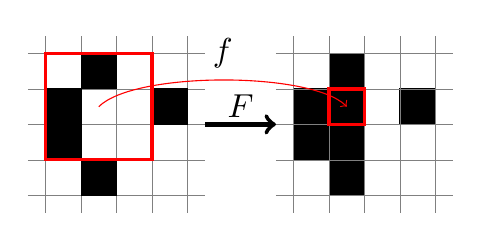
\begin{tikzpicture}[scale=0.45, every node/.style={scale=1.2}]]
\draw [fill] (2,10) rectangle (3,9);
\draw [fill] (2,11) rectangle (3,10);
\draw [fill] (2,9) rectangle (3,8);
\draw [fill] (1,10) rectangle (2,8) node (v2) {};
\draw [fill] (v2) rectangle (3,7);
\draw [fill] (4,10) rectangle (5,9);

\draw [-][help lines, step=1cm] (-6.5,6.5) grid (-1.5,11.5);
\draw [-][help lines, step=1cm] (0.5,6.5) grid (5.5,11.5);
\draw [fill=black] (-5,11) rectangle (-4,10);
\draw [fill=black] (-6,10) rectangle (-5,9);
\draw [fill=black] (-6,9) rectangle (-5,8);
\draw [fill=black] (-4,8) rectangle (-5,7);
\draw [fill=black] (-3,10) rectangle (-2,9);
\draw [->,ultra thick](-1.5,9) -- (0.5,9);
\node at (-0.5,9.5) {$F$};
\draw [red,very thick] (-6,11) rectangle (-3,8);
\draw [red,very thick,fill=black] (2,10) rectangle (3,9);
\draw [red,->](-4.5,9.5) .. controls (-3.5,10.5) and (1.5,10.5) .. (2.5,9.5);
\node at (-1,11) {$f$};
\end{tikzpicture}
\end{center}
% \end{minipage}
\hfill
% \begin{minipage}[c]{0.5\textwidth}
% \centering
% \begin{center}
%   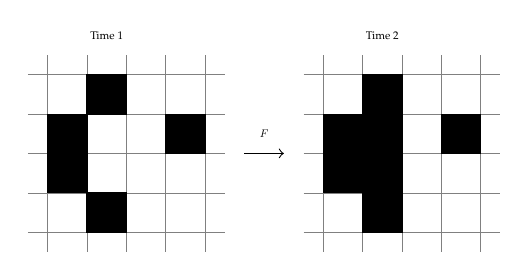
\begin{tikzpicture}[scale=0.5, every node/.style={scale=0.4}]]
%\draw [fill,gray!10] (0.5,2.5) rectangle (5.5,-2.5);
\draw [-][help lines, step=1cm] (-6.5,-2.5) grid (-1.5,2.5);
\draw [-][help lines, step=1cm] (0.5,-2.5) grid (5.5,2.5);
\draw [fill=black] (-5,2) rectangle (-4,1);
\draw [fill=black] (-6,1) rectangle (-5,0);
\draw [fill=black] (-6,0) rectangle (-5,-1);
\draw [fill=black] (-4,-1) rectangle (-5,-2);
\draw [fill=black] (-3,1) rectangle (-2,0);
\draw [->](-1,0) -- (0,0);
\node at (-0.5,0.5) {$F$};
%\draw [red,very thick] (-6,1) rectangle (-3,-2);
%\draw [red,very thick,fill=black] (2,0) rectangle (3,-1);
%\draw [red,->](-4.5,-0.5) .. controls (-3.5,0.5) and (1.5,0.5) .. (2.5,-0.5);
%\node at (-1,0.5) {$f$};

\node at (-4.5,3) {Time 1};
\node at (2.5,3) {Time 2};

\draw [fill] (2,1) rectangle (3,0);
%\draw [fill=white] (3,1) node (v1) {} rectangle (4,0);
%\draw [fill=white] (3,0) rectangle (4,-1);
\draw [fill] (2,2) rectangle (3,1);
\draw [fill] (2,0) rectangle (3,-1);
\draw [fill] (1,1) rectangle (2,-1) node (v2) {};
\draw [fill] (v2) rectangle (3,-2);
\draw [fill] (4,1) rectangle (5,0);
\end{tikzpicture}
% \end{center}
% \end{minipage}
\hfill
  } 
%%%%%%%%%%%%%%%%%%%%%%%%%%%%%%%%%%%%%%%%%%%%%%%%%%%%%%%%%%%%%%%%%%%%%%%%%%%%%%%%%%%%%%%%%%%%%%%%%%%%%%%%%%%%%%%%%%%%%%%%%%%%%%%%%%%%%%%%%%%%%%%%%%%%%%%%%%%%
  \headerbox{Freezing}{name=freezing,column=0,span=2,row=1,below=def}{
%%%%%%%%%%%%%%%%%%%%%%%%%%%%%%%%%%%%%%%%%%%%%%%%%%%%%%%%%%%%%%%%%%%%%%%%%%%%%%%%%%%%%%%%%%%%%%%%%%%%%%%%%%%%%%%%%%%%%%%%%%%%%%%%%%%%%%%%%%%%%%%%%%%%%%%%%%%%
A {\emph{ freezing CA}} (FCA) is a CA $F$ compatible with a partial order $\geqslant$ on states:
    \begin{align*}
    F(c)_z\geqslant c_z\qquad\forall z\in \mathbb{Z}^2 \quad\forall c\in Q^{\mathbb{Z}^2}
    \end{align*}

{\bf Example:} Life without death.

 }
%%%%%%%%%%%%%%%%%%%%%%%%%%%%%%%%%%%%%%%%%%%%%%%%%%%%%%%%%%%%%%%%%%%%%%%%%%%%%%%%%%%%%%%%%%%%%%%%%%%%%%%%%%%%%%%%%%%%%%%%%%%%%%%%%%%%%%%%%%%%%%%%%%%%%%%%%%%%
  \headerbox{Freezing+Totalistic}{name=f+t,column=2,span=2,row=0}{
%%%%%%%%%%%%%%%%%%%%%%%%%%%%%%%%%%%%%%%%%%%%%%%%%%%%%%%%%%%%%%%%%%%%%%%%%%%%%%%%%%%%%%%%%%%%%%%%%%%%%%%%%%%%%%%%%%%%%%%%%%%%%%%%%%%%%%%%%%%%%%%%%%%%%%%%%%%%
\begin{flushleft}
\noindent The family of FTCA with 2 states and five neighbors is given by:
\end{flushleft} 
\vspace*{-15pt}
% \begin{minipage}{0.4\textwidth}
%     \begin{center}
%       Freezing + Totalistic \\+ 2D +\\ 2 states + Von Neumann  
%     \end{center}
% \end{minipage}   
% \begin{minipage}{0.025\textwidth}
%     \begin{center}
%       =  
%     \end{center}
% \end{minipage}  
% \begin{minipage}{0.325\textwidth}
%     \begin{center}
%       CA that only change from 0 to 1 depending on the sum of its neighbors.  
%     \end{center}
% \end{minipage}
\hspace*{-5pt}
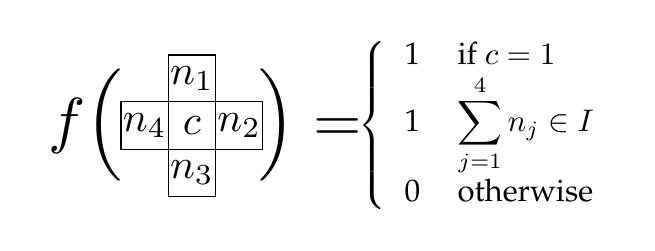
\begin{tikzpicture}[scale=0.6, every node/.style={scale=1.5}]]
\draw  (-0.9928,1.9927) rectangle (0,-1);
\draw  (-2,1) rectangle (1,0);
\node[scale=1.5, every node/.style={scale=1.5}] at (-2.75,0.5) {$f\Big($};
\node[scale=1.5, every node/.style={scale=1.5}] at (2.0,0.5)    {$ \Big)=$};
\node at (-0.5,1.5) {$n_1$};
\node at ( 0.5,0.5) {$n_2$};
\node at (-0.5,-0.5) {$n_3$};
\node at (-1.5,0.5) {$n_4$};
\node at (-0.5,0.5) {$c$};
\node[scale=0.75, every node/.style={scale=0.75}] at (5.75,0.5)    {$\left\{
  \begin{tabular}{rl}
  1 & if $c=1$\\
  1 & $\displaystyle\sum_{j=1}^4 n_j\in I$\\
  0 & otherwise
  \end{tabular}
\right.$};
\end{tikzpicture}
Where $I\subseteq\{0,1,2,3,4\} $.
\vspace*{-10pt}
\begin{description}
  \item[Notation:]  We call a TFCA by a number, representing the elements of $I$. \vspace*{-7.5pt}
  \item[] There are 32 possible TFCA.\vspace*{-7.5pt}
  \item[Example] The TFCA 24 is the TFCA that change to 1 with exactly 2 or 4 neighbors in state 1.
\end{description}


 }
%%%%%%%%%%%%%%%%%%%%%%%%%%%%%%%%%%%%%%%%%%%%%%%%%%%%%%%%%%%%%%%%%%%%%%%%%%%%%%%%%%%%%%%%%%%%%%%%%%%%%%%%%%%%%%%%%%%%%%%%%%%%%%%%%%%%%%%%%%%%%%%%%%%%%%%%%%%%
  \headerbox{Totalistic}{name=totalistic,column=4,span=2,row=1,below=def}{
%%%%%%%%%%%%%%%%%%%%%%%%%%%%%%%%%%%%%%%%%%%%%%%%%%%%%%%%%%%%%%%%%%%%%%%%%%%%%%%%%%%%%%%%%%%%%%%%%%%%%%%%%%%%%%%%%%%%%%%%%%%%%%%%%%%%%%%%%%%%%%%%%%%%%%%%%%%%
A {\emph{ totalistic CA}} (TCA) is a CA $F$ where the LF only depend of the center cell and the total neighborhood:
\begin{align*}
\displaystyle F(c)_z=f\left(c_z,\sum_{z\in N} c_z\right)\quad\forall z\in \mathbb{Z}^d, \ \forall c\in Q^{\mathbb{Z}^d}
\end{align*}
{\bf Example:} Life without death.
 }
%%%%%%%%%%%%%%%%%%%%%%%%%%%%%%%%%%%%%%%%%%%%%%%%%%%%%%%%%%%%%%%%%%%%%%%%%%%%%%%%%%%%%%%%%%%%%%%%%%%%%%%%%%%%%%%%%%%%%%%%%%%%%%%%%%%%%%%%%%%%%%%%%%%%%%%%%%%%
  \headerbox{Dynamics, fifth iteration }{name=ex,column=0,span=6,row=2,below=freezing}{
%%%%%%%%%%%%%%%%%%%%%%%%%%%%%%%%%%%%%%%%%%%%%%%%%%%%%%%%%%%%%%%%%%%%%%%%%%%%%%%%%%%%%%%%%%%%%%%%%%%%%%%%%%%%%%%%%%%%%%%%%%%%%%%%%%%%%%%%%%%%%%%%%%%%%%%%%%%%

\begin{center}
\hfill
        \begin{minipage}{0.065\textwidth}
            \begin{center}
            \begin{tikzpicture}[scale=0.15]
              % Para incluir 4_1.tex en un doc LaTeX se puede insertar el siguiente codigo:

% \usepackage{tikz}
% \usepackage{pgffor}
% 
% \foreach \n in {1,...,5}{
% \only<\n>{
% \begin{center} 
% 	\begin{tikzpicture}[scale=1.0]
% 		\input{./4/4_\n}
% 	\end{tikzpicture}
% \end{center}}}

\fill[black] (8,8) rectangle (9,9); 
\fill[black] (9,7) rectangle (10,8); 
\fill[black] (6,6) rectangle (7,7); 
\fill[black] (3,5) rectangle (4,6); 
\fill[black] (5,5) rectangle (6,6); 
\fill[black] (7,5) rectangle (8,6); 
\fill[black] (4,4) rectangle (5,5); 
\fill[black] (6,4) rectangle (7,5); 
\fill[black] (7,1) rectangle (8,2); 

\draw[color=gray, thick] (1,1) grid (11,11);
\draw[color=black, thick] (1,1) rectangle (11,11);
 % Seleccionar 28x28 celdas en golly
            \end{tikzpicture} 
            \small{Initial}           
            \end{center}
        \end{minipage}   
\hfill
        \begin{minipage}{0.065\textwidth}
            \begin{center}
            \begin{tikzpicture}[scale=0.15]
              % Para incluir 4_5.tex en un doc LaTeX se puede insertar el siguiente codigo:

% \usepackage{tikz}
% \usepackage{pgffor}
% 
% \foreach \n in {1,...,5}{
% \only<\n>{
% \begin{center} 
% 	\begin{tikzpicture}[scale=1.0]
% 		\input{./4/4_\n}
% 	\end{tikzpicture}
% \end{center}}}

\fill[black] (8,8) rectangle (9,9); 
\fill[black] (9,7) rectangle (10,8); 
\fill[black] (6,6) rectangle (7,7); 
\fill[black] (3,5) rectangle (4,6); 
\fill[black] (5,5) rectangle (6,6); 
\fill[black] (6,5) rectangle (7,6); 
\fill[black] (7,5) rectangle (8,6); 
\fill[black] (4,4) rectangle (5,5); 
\fill[black] (6,4) rectangle (7,5); 
\fill[black] (7,1) rectangle (8,2); 

\draw[color=gray, thick] (1,1) grid (11,11);
\draw[color=black, thick] (1,1) rectangle (11,11);
 % Seleccionar 28x28 celdas en golly
            \end{tikzpicture} 
            \small{Rule 4}           
            \end{center}
        \end{minipage}   
 \hfill        
        \begin{minipage}{0.065\textwidth}
            \begin{center}
            \begin{tikzpicture}[scale=0.15]
              % Para incluir 3_5.tex en un doc LaTeX se puede insertar el siguiente codigo:

% \usepackage{tikz}
% \usepackage{pgffor}
% 
% \foreach \n in {1,...,5}{
% \only<\n>{
% \begin{center} 
% 	\begin{tikzpicture}[scale=1.0]
% 		\input{./3/3_\n}
% 	\end{tikzpicture}
% \end{center}}}

\fill[black] (8,8) rectangle (9,9); 
\fill[black] (9,7) rectangle (10,8); 
\fill[black] (6,6) rectangle (7,7); 
\fill[black] (3,5) rectangle (4,6); 
\fill[black] (4,5) rectangle (5,6); 
\fill[black] (5,5) rectangle (6,6); 
\fill[black] (7,5) rectangle (8,6); 
\fill[black] (4,4) rectangle (5,5); 
\fill[black] (5,4) rectangle (6,5); 
\fill[black] (6,4) rectangle (7,5); 
\fill[black] (7,1) rectangle (8,2); 

\draw[color=gray, thick] (1,1) grid (11,11);
\draw[color=black, thick] (1,1) rectangle (11,11);
 % Seleccionar 28x28 celdas en golly
            \end{tikzpicture}

            \small{Rule 3}
            \end{center}            
        \end{minipage}
\hfill
        \begin{minipage}{0.065\textwidth}
            \begin{center}
            \begin{tikzpicture}[scale=0.15]
              % Para incluir 34_5.tex en un doc LaTeX se puede insertar el siguiente codigo:

% \usepackage{tikz}
% \usepackage{pgffor}
% 
% \foreach \n in {1,...,5}{
% \only<\n>{
% \begin{center} 
% 	\begin{tikzpicture}[scale=1.0]
% 		\input{./34/34_\n}
% 	\end{tikzpicture}
% \end{center}}}

\fill[black] (8,8) rectangle (9,9); 
\fill[black] (9,7) rectangle (10,8); 
\fill[black] (6,6) rectangle (7,7); 
\fill[black] (3,5) rectangle (4,6); 
\fill[black] (4,5) rectangle (5,6); 
\fill[black] (5,5) rectangle (6,6); 
\fill[black] (6,5) rectangle (7,6); 
\fill[black] (7,5) rectangle (8,6); 
\fill[black] (4,4) rectangle (5,5); 
\fill[black] (5,4) rectangle (6,5); 
\fill[black] (6,4) rectangle (7,5); 
\fill[black] (7,1) rectangle (8,2); 

\draw[color=gray, thick] (1,1) grid (11,11);
\draw[color=black, thick] (1,1) rectangle (11,11);
 % Seleccionar 28x28 celdas en golly
            \end{tikzpicture}

            \small{Rule 34}
            \end{center}            
        \end{minipage}
\hfill
        \begin{minipage}{0.065\textwidth}
            \begin{center}
            \begin{tikzpicture}[scale=0.15]
              % Para incluir 2_5.tex en un doc LaTeX se puede insertar el siguiente codigo:

% \usepackage{tikz}
% \usepackage{pgffor}
% 
% \foreach \n in {1,...,5}{
% \only<\n>{
% \begin{center} 
% 	\begin{tikzpicture}[scale=1.0]
% 		\input{./2/2_\n}
% 	\end{tikzpicture}
% \end{center}}}

\fill[black] (6,8) rectangle (7,9); 
\fill[black] (7,8) rectangle (8,9); 
\fill[black] (8,8) rectangle (9,9); 
\fill[black] (9,8) rectangle (10,9); 
\fill[black] (5,7) rectangle (6,8); 
\fill[black] (6,7) rectangle (7,8); 
\fill[black] (7,7) rectangle (8,8); 
\fill[black] (8,7) rectangle (9,8); 
\fill[black] (9,7) rectangle (10,8); 
\fill[black] (5,6) rectangle (6,7); 
\fill[black] (6,6) rectangle (7,7); 
\fill[black] (7,6) rectangle (8,7); 
\fill[black] (8,6) rectangle (9,7); 
\fill[black] (9,6) rectangle (10,7); 
\fill[black] (3,5) rectangle (4,6); 
\fill[black] (5,5) rectangle (6,6); 
\fill[black] (7,5) rectangle (8,6); 
\fill[black] (8,5) rectangle (9,6); 
\fill[black] (9,5) rectangle (10,6); 
\fill[black] (3,4) rectangle (4,5); 
\fill[black] (4,4) rectangle (5,5); 
\fill[black] (6,4) rectangle (7,5); 
\fill[black] (7,4) rectangle (8,5); 
\fill[black] (8,4) rectangle (9,5); 
\fill[black] (7,1) rectangle (8,2); 

\draw[color=gray, thick] (1,1) grid (11,11);
\draw[color=black, thick] (1,1) rectangle (11,11);
 % Seleccionar 28x28 celdas en golly
            \end{tikzpicture}

            \small{Rule 2}
            \end{center}            
        \end{minipage}
\hfill
        \begin{minipage}{0.065\textwidth}
            \begin{center}
            \begin{tikzpicture}[scale=0.15]
              % Para incluir 24_5.tex en un doc LaTeX se puede insertar el siguiente codigo:

% \usepackage{tikz}
% \usepackage{pgffor}
% 
% \foreach \n in {1,...,5}{
% \only<\n>{
% \begin{center} 
% 	\begin{tikzpicture}[scale=1.0]
% 		\input{./24/24_\n}
% 	\end{tikzpicture}
% \end{center}}}

\fill[black] (6,8) rectangle (7,9); 
\fill[black] (7,8) rectangle (8,9); 
\fill[black] (8,8) rectangle (9,9); 
\fill[black] (9,8) rectangle (10,9); 
\fill[black] (5,7) rectangle (6,8); 
\fill[black] (6,7) rectangle (7,8); 
\fill[black] (7,7) rectangle (8,8); 
\fill[black] (8,7) rectangle (9,8); 
\fill[black] (9,7) rectangle (10,8); 
\fill[black] (5,6) rectangle (6,7); 
\fill[black] (6,6) rectangle (7,7); 
\fill[black] (7,6) rectangle (8,7); 
\fill[black] (8,6) rectangle (9,7); 
\fill[black] (9,6) rectangle (10,7); 
\fill[black] (3,5) rectangle (4,6); 
\fill[black] (5,5) rectangle (6,6); 
\fill[black] (6,5) rectangle (7,6); 
\fill[black] (7,5) rectangle (8,6); 
\fill[black] (8,5) rectangle (9,6); 
\fill[black] (9,5) rectangle (10,6); 
\fill[black] (3,4) rectangle (4,5); 
\fill[black] (4,4) rectangle (5,5); 
\fill[black] (6,4) rectangle (7,5); 
\fill[black] (7,4) rectangle (8,5); 
\fill[black] (8,4) rectangle (9,5); 
\fill[black] (7,1) rectangle (8,2); 

\draw[color=gray, thick] (1,1) grid (11,11);
\draw[color=black, thick] (1,1) rectangle (11,11);
 % Seleccionar 28x28 celdas en golly
            \end{tikzpicture}

            \small{Rule 24}
            \end{center}            
        \end{minipage}
\hfill
        \begin{minipage}{0.065\textwidth}
            \begin{center}
            \begin{tikzpicture}[scale=0.15]
              % Para incluir 23_5.tex en un doc LaTeX se puede insertar el siguiente codigo:

% \usepackage{tikz}
% \usepackage{pgffor}
% 
% \foreach \n in {1,...,5}{
% \only<\n>{
% \begin{center} 
% 	\begin{tikzpicture}[scale=1.0]
% 		\input{./23/23_\n}
% 	\end{tikzpicture}
% \end{center}}}

\fill[black] (6,8) rectangle (7,9); 
\fill[black] (7,8) rectangle (8,9); 
\fill[black] (8,8) rectangle (9,9); 
\fill[black] (9,8) rectangle (10,9); 
\fill[black] (5,7) rectangle (6,8); 
\fill[black] (6,7) rectangle (7,8); 
\fill[black] (7,7) rectangle (8,8); 
\fill[black] (8,7) rectangle (9,8); 
\fill[black] (9,7) rectangle (10,8); 
\fill[black] (3,6) rectangle (4,7); 
\fill[black] (4,6) rectangle (5,7); 
\fill[black] (5,6) rectangle (6,7); 
\fill[black] (6,6) rectangle (7,7); 
\fill[black] (7,6) rectangle (8,7); 
\fill[black] (8,6) rectangle (9,7); 
\fill[black] (9,6) rectangle (10,7); 
\fill[black] (3,5) rectangle (4,6); 
\fill[black] (4,5) rectangle (5,6); 
\fill[black] (5,5) rectangle (6,6); 
\fill[black] (7,5) rectangle (8,6); 
\fill[black] (8,5) rectangle (9,6); 
\fill[black] (9,5) rectangle (10,6); 
\fill[black] (3,4) rectangle (4,5); 
\fill[black] (4,4) rectangle (5,5); 
\fill[black] (5,4) rectangle (6,5); 
\fill[black] (6,4) rectangle (7,5); 
\fill[black] (7,4) rectangle (8,5); 
\fill[black] (8,4) rectangle (9,5); 
\fill[black] (7,1) rectangle (8,2); 

\draw[color=gray, thick] (1,1) grid (11,11);
\draw[color=black, thick] (1,1) rectangle (11,11);
 % Seleccionar 28x28 celdas en golly
            \end{tikzpicture}

            \small{Rule 23}
            \end{center}            
        \end{minipage}
\hfill
        \begin{minipage}{0.065\textwidth}
            \begin{center}
            \begin{tikzpicture}[scale=0.15]
              % Para incluir 234_5.tex en un doc LaTeX se puede insertar el siguiente codigo:

% \usepackage{tikz}
% \usepackage{pgffor}
% 
% \foreach \n in {1,...,5}{
% \only<\n>{
% \begin{center} 
% 	\begin{tikzpicture}[scale=1.0]
% 		\input{./234/234_\n}
% 	\end{tikzpicture}
% \end{center}}}

\fill[black] (6,8) rectangle (7,9); 
\fill[black] (7,8) rectangle (8,9); 
\fill[black] (8,8) rectangle (9,9); 
\fill[black] (9,8) rectangle (10,9); 
\fill[black] (5,7) rectangle (6,8); 
\fill[black] (6,7) rectangle (7,8); 
\fill[black] (7,7) rectangle (8,8); 
\fill[black] (8,7) rectangle (9,8); 
\fill[black] (9,7) rectangle (10,8); 
\fill[black] (3,6) rectangle (4,7); 
\fill[black] (4,6) rectangle (5,7); 
\fill[black] (5,6) rectangle (6,7); 
\fill[black] (6,6) rectangle (7,7); 
\fill[black] (7,6) rectangle (8,7); 
\fill[black] (8,6) rectangle (9,7); 
\fill[black] (9,6) rectangle (10,7); 
\fill[black] (3,5) rectangle (4,6); 
\fill[black] (4,5) rectangle (5,6); 
\fill[black] (5,5) rectangle (6,6); 
\fill[black] (6,5) rectangle (7,6); 
\fill[black] (7,5) rectangle (8,6); 
\fill[black] (8,5) rectangle (9,6); 
\fill[black] (9,5) rectangle (10,6); 
\fill[black] (3,4) rectangle (4,5); 
\fill[black] (4,4) rectangle (5,5); 
\fill[black] (5,4) rectangle (6,5); 
\fill[black] (6,4) rectangle (7,5); 
\fill[black] (7,4) rectangle (8,5); 
\fill[black] (8,4) rectangle (9,5); 
\fill[black] (7,1) rectangle (8,2); 

\draw[color=gray, thick] (1,1) grid (11,11);
\draw[color=black, thick] (1,1) rectangle (11,11);
 % Seleccionar 28x28 celdas en golly
            \end{tikzpicture}
            \small{Rule 234}
            \end{center}            
        \end{minipage}
\hfill {\color[rgb]{1,1,1} .}

\hfill
        \begin{minipage}{0.065\textwidth}
            \begin{center}
            \begin{tikzpicture}[scale=0.15]
              % Para incluir 1_5.tex en un doc LaTeX se puede insertar el siguiente codigo:

% \usepackage{tikz}
% \usepackage{pgffor}
% 
% \foreach \n in {1,...,5}{
% \only<\n>{
% \begin{center} 
% 	\begin{tikzpicture}[scale=1.0]
% 		\input{./1/1_\n}
% 	\end{tikzpicture}
% \end{center}}}

\fill[black] (6,10) rectangle (7,11); 
\fill[black] (7,10) rectangle (8,11); 
\fill[black] (8,10) rectangle (9,11); 
\fill[black] (3,9) rectangle (4,10); 
\fill[black] (5,9) rectangle (6,10); 
\fill[black] (8,9) rectangle (9,10); 
\fill[black] (9,9) rectangle (10,10); 
\fill[black] (3,8) rectangle (4,9); 
\fill[black] (5,8) rectangle (6,9); 
\fill[black] (7,8) rectangle (8,9); 
\fill[black] (8,8) rectangle (9,9); 
\fill[black] (10,8) rectangle (11,9); 
\fill[black] (2,7) rectangle (3,8); 
\fill[black] (3,7) rectangle (4,8); 
\fill[black] (5,7) rectangle (6,8); 
\fill[black] (6,7) rectangle (7,8); 
\fill[black] (9,7) rectangle (10,8); 
\fill[black] (10,7) rectangle (11,8); 
\fill[black] (1,6) rectangle (2,7); 
\fill[black] (3,6) rectangle (4,7); 
\fill[black] (4,6) rectangle (5,7); 
\fill[black] (6,6) rectangle (7,7); 
\fill[black] (9,6) rectangle (10,7); 
\fill[black] (1,5) rectangle (2,6); 
\fill[black] (2,5) rectangle (3,6); 
\fill[black] (3,5) rectangle (4,6); 
\fill[black] (5,5) rectangle (6,6); 
\fill[black] (7,5) rectangle (8,6); 
\fill[black] (8,5) rectangle (9,6); 
\fill[black] (2,4) rectangle (3,5); 
\fill[black] (4,4) rectangle (5,5); 
\fill[black] (6,4) rectangle (7,5); 
\fill[black] (8,4) rectangle (9,5); 
\fill[black] (9,4) rectangle (10,5); 
\fill[black] (10,4) rectangle (11,5); 
\fill[black] (3,3) rectangle (4,4); 
\fill[black] (4,3) rectangle (5,4); 
\fill[black] (6,3) rectangle (7,4); 
\fill[black] (8,3) rectangle (9,4); 
\fill[black] (4,2) rectangle (5,3); 
\fill[black] (7,2) rectangle (8,3); 
\fill[black] (9,2) rectangle (10,3); 
\fill[black] (5,1) rectangle (6,2); 
\fill[black] (6,1) rectangle (7,2); 
\fill[black] (7,1) rectangle (8,2); 
\fill[black] (8,1) rectangle (9,2); 
\fill[black] (9,1) rectangle (10,2); 
\fill[black] (10,1) rectangle (11,2); 

\draw[color=gray, thick] (1,1) grid (11,11);
\draw[color=black, thick] (1,1) rectangle (11,11);
 % Seleccionar 28x28 celdas en golly
            \end{tikzpicture}
            \small{Rule 1}
            \end{center}            
        \end{minipage}
\hfill
        \begin{minipage}{0.065\textwidth}
            \begin{center}
            \begin{tikzpicture}[scale=0.15]
              % Para incluir 14_5.tex en un doc LaTeX se puede insertar el siguiente codigo:

% \usepackage{tikz}
% \usepackage{pgffor}
% 
% \foreach \n in {1,...,5}{
% \only<\n>{
% \begin{center} 
% 	\begin{tikzpicture}[scale=1.0]
% 		\input{./14/14_\n}
% 	\end{tikzpicture}
% \end{center}}}

\fill[black] (6,10) rectangle (7,11); 
\fill[black] (7,10) rectangle (8,11); 
\fill[black] (8,10) rectangle (9,11); 
\fill[black] (3,9) rectangle (4,10); 
\fill[black] (5,9) rectangle (6,10); 
\fill[black] (8,9) rectangle (9,10); 
\fill[black] (9,9) rectangle (10,10); 
\fill[black] (3,8) rectangle (4,9); 
\fill[black] (5,8) rectangle (6,9); 
\fill[black] (7,8) rectangle (8,9); 
\fill[black] (8,8) rectangle (9,9); 
\fill[black] (9,8) rectangle (10,9); 
\fill[black] (10,8) rectangle (11,9); 
\fill[black] (2,7) rectangle (3,8); 
\fill[black] (3,7) rectangle (4,8); 
\fill[black] (5,7) rectangle (6,8); 
\fill[black] (6,7) rectangle (7,8); 
\fill[black] (9,7) rectangle (10,8); 
\fill[black] (10,7) rectangle (11,8); 
\fill[black] (1,6) rectangle (2,7); 
\fill[black] (2,6) rectangle (3,7); 
\fill[black] (3,6) rectangle (4,7); 
\fill[black] (4,6) rectangle (5,7); 
\fill[black] (5,6) rectangle (6,7); 
\fill[black] (6,6) rectangle (7,7); 
\fill[black] (9,6) rectangle (10,7); 
\fill[black] (1,5) rectangle (2,6); 
\fill[black] (2,5) rectangle (3,6); 
\fill[black] (3,5) rectangle (4,6); 
\fill[black] (4,5) rectangle (5,6); 
\fill[black] (5,5) rectangle (6,6); 
\fill[black] (6,5) rectangle (7,6); 
\fill[black] (7,5) rectangle (8,6); 
\fill[black] (8,5) rectangle (9,6); 
\fill[black] (2,4) rectangle (3,5); 
\fill[black] (3,4) rectangle (4,5); 
\fill[black] (4,4) rectangle (5,5); 
\fill[black] (6,4) rectangle (7,5); 
\fill[black] (8,4) rectangle (9,5); 
\fill[black] (9,4) rectangle (10,5); 
\fill[black] (10,4) rectangle (11,5); 
\fill[black] (3,3) rectangle (4,4); 
\fill[black] (4,3) rectangle (5,4); 
\fill[black] (6,3) rectangle (7,4); 
\fill[black] (8,3) rectangle (9,4); 
\fill[black] (4,2) rectangle (5,3); 
\fill[black] (7,2) rectangle (8,3); 
\fill[black] (8,2) rectangle (9,3); 
\fill[black] (9,2) rectangle (10,3); 
\fill[black] (5,1) rectangle (6,2); 
\fill[black] (6,1) rectangle (7,2); 
\fill[black] (7,1) rectangle (8,2); 
\fill[black] (8,1) rectangle (9,2); 
\fill[black] (9,1) rectangle (10,2); 
\fill[black] (10,1) rectangle (11,2); 

\draw[color=gray, thick] (1,1) grid (11,11);
\draw[color=black, thick] (1,1) rectangle (11,11);
 % Seleccionar 28x28 celdas en golly
            \end{tikzpicture}
            \small{Rule 14}
            \end{center}            
        \end{minipage}
\hfill
        \begin{minipage}{0.065\textwidth}
            \begin{center}
            \begin{tikzpicture}[scale=0.15]
              % Para incluir 13_5.tex en un doc LaTeX se puede insertar el siguiente codigo:

% \usepackage{tikz}
% \usepackage{pgffor}
% 
% \foreach \n in {1,...,5}{
% \only<\n>{
% \begin{center} 
% 	\begin{tikzpicture}[scale=1.0]
% 		\input{./13/13_\n}
% 	\end{tikzpicture}
% \end{center}}}

\fill[black] (6,10) rectangle (7,11); 
\fill[black] (7,10) rectangle (8,11); 
\fill[black] (8,10) rectangle (9,11); 
\fill[black] (3,9) rectangle (4,10); 
\fill[black] (5,9) rectangle (6,10); 
\fill[black] (7,9) rectangle (8,10); 
\fill[black] (8,9) rectangle (9,10); 
\fill[black] (9,9) rectangle (10,10); 
\fill[black] (3,8) rectangle (4,9); 
\fill[black] (5,8) rectangle (6,9); 
\fill[black] (6,8) rectangle (7,9); 
\fill[black] (7,8) rectangle (8,9); 
\fill[black] (8,8) rectangle (9,9); 
\fill[black] (10,8) rectangle (11,9); 
\fill[black] (2,7) rectangle (3,8); 
\fill[black] (3,7) rectangle (4,8); 
\fill[black] (5,7) rectangle (6,8); 
\fill[black] (6,7) rectangle (7,8); 
\fill[black] (9,7) rectangle (10,8); 
\fill[black] (10,7) rectangle (11,8); 
\fill[black] (1,6) rectangle (2,7); 
\fill[black] (3,6) rectangle (4,7); 
\fill[black] (4,6) rectangle (5,7); 
\fill[black] (5,6) rectangle (6,7); 
\fill[black] (6,6) rectangle (7,7); 
\fill[black] (9,6) rectangle (10,7); 
\fill[black] (10,6) rectangle (11,7); 
\fill[black] (1,5) rectangle (2,6); 
\fill[black] (2,5) rectangle (3,6); 
\fill[black] (3,5) rectangle (4,6); 
\fill[black] (4,5) rectangle (5,6); 
\fill[black] (5,5) rectangle (6,6); 
\fill[black] (7,5) rectangle (8,6); 
\fill[black] (8,5) rectangle (9,6); 
\fill[black] (9,5) rectangle (10,6); 
\fill[black] (2,4) rectangle (3,5); 
\fill[black] (4,4) rectangle (5,5); 
\fill[black] (5,4) rectangle (6,5); 
\fill[black] (6,4) rectangle (7,5); 
\fill[black] (7,4) rectangle (8,5); 
\fill[black] (8,4) rectangle (9,5); 
\fill[black] (9,4) rectangle (10,5); 
\fill[black] (10,4) rectangle (11,5); 
\fill[black] (3,3) rectangle (4,4); 
\fill[black] (4,3) rectangle (5,4); 
\fill[black] (5,3) rectangle (6,4); 
\fill[black] (6,3) rectangle (7,4); 
\fill[black] (8,3) rectangle (9,4); 
\fill[black] (9,3) rectangle (10,4); 
\fill[black] (4,2) rectangle (5,3); 
\fill[black] (6,2) rectangle (7,3); 
\fill[black] (7,2) rectangle (8,3); 
\fill[black] (9,2) rectangle (10,3); 
\fill[black] (5,1) rectangle (6,2); 
\fill[black] (6,1) rectangle (7,2); 
\fill[black] (7,1) rectangle (8,2); 
\fill[black] (8,1) rectangle (9,2); 
\fill[black] (9,1) rectangle (10,2); 
\fill[black] (10,1) rectangle (11,2); 

\draw[color=gray, thick] (1,1) grid (11,11);
\draw[color=black, thick] (1,1) rectangle (11,11);
 % Seleccionar 28x28 celdas en golly
            \end{tikzpicture}
            \small{Rule 13}
            \end{center}            
        \end{minipage}
\hfill      
        \begin{minipage}{0.065\textwidth}
            \begin{center}
            \begin{tikzpicture}[scale=0.15]
              % Para incluir 134_5.tex en un doc LaTeX se puede insertar el siguiente codigo:

% \usepackage{tikz}
% \usepackage{pgffor}
% 
% \foreach \n in {1,...,5}{
% \only<\n>{
% \begin{center} 
% 	\begin{tikzpicture}[scale=1.0]
% 		\input{./134/134_\n}
% 	\end{tikzpicture}
% \end{center}}}

\fill[black] (6,10) rectangle (7,11); 
\fill[black] (7,10) rectangle (8,11); 
\fill[black] (8,10) rectangle (9,11); 
\fill[black] (3,9) rectangle (4,10); 
\fill[black] (5,9) rectangle (6,10); 
\fill[black] (7,9) rectangle (8,10); 
\fill[black] (8,9) rectangle (9,10); 
\fill[black] (9,9) rectangle (10,10); 
\fill[black] (3,8) rectangle (4,9); 
\fill[black] (5,8) rectangle (6,9); 
\fill[black] (6,8) rectangle (7,9); 
\fill[black] (7,8) rectangle (8,9); 
\fill[black] (8,8) rectangle (9,9); 
\fill[black] (9,8) rectangle (10,9); 
\fill[black] (10,8) rectangle (11,9); 
\fill[black] (2,7) rectangle (3,8); 
\fill[black] (3,7) rectangle (4,8); 
\fill[black] (5,7) rectangle (6,8); 
\fill[black] (6,7) rectangle (7,8); 
\fill[black] (9,7) rectangle (10,8); 
\fill[black] (10,7) rectangle (11,8); 
\fill[black] (1,6) rectangle (2,7); 
\fill[black] (2,6) rectangle (3,7); 
\fill[black] (3,6) rectangle (4,7); 
\fill[black] (4,6) rectangle (5,7); 
\fill[black] (5,6) rectangle (6,7); 
\fill[black] (6,6) rectangle (7,7); 
\fill[black] (9,6) rectangle (10,7); 
\fill[black] (10,6) rectangle (11,7); 
\fill[black] (1,5) rectangle (2,6); 
\fill[black] (2,5) rectangle (3,6); 
\fill[black] (3,5) rectangle (4,6); 
\fill[black] (4,5) rectangle (5,6); 
\fill[black] (5,5) rectangle (6,6); 
\fill[black] (6,5) rectangle (7,6); 
\fill[black] (7,5) rectangle (8,6); 
\fill[black] (8,5) rectangle (9,6); 
\fill[black] (9,5) rectangle (10,6); 
\fill[black] (2,4) rectangle (3,5); 
\fill[black] (3,4) rectangle (4,5); 
\fill[black] (4,4) rectangle (5,5); 
\fill[black] (5,4) rectangle (6,5); 
\fill[black] (6,4) rectangle (7,5); 
\fill[black] (7,4) rectangle (8,5); 
\fill[black] (8,4) rectangle (9,5); 
\fill[black] (9,4) rectangle (10,5); 
\fill[black] (10,4) rectangle (11,5); 
\fill[black] (3,3) rectangle (4,4); 
\fill[black] (4,3) rectangle (5,4); 
\fill[black] (5,3) rectangle (6,4); 
\fill[black] (6,3) rectangle (7,4); 
\fill[black] (7,3) rectangle (8,4); 
\fill[black] (8,3) rectangle (9,4); 
\fill[black] (9,3) rectangle (10,4); 
\fill[black] (4,2) rectangle (5,3); 
\fill[black] (5,2) rectangle (6,3); 
\fill[black] (6,2) rectangle (7,3); 
\fill[black] (7,2) rectangle (8,3); 
\fill[black] (8,2) rectangle (9,3); 
\fill[black] (9,2) rectangle (10,3); 
\fill[black] (5,1) rectangle (6,2); 
\fill[black] (6,1) rectangle (7,2); 
\fill[black] (7,1) rectangle (8,2); 
\fill[black] (8,1) rectangle (9,2); 
\fill[black] (9,1) rectangle (10,2); 
\fill[black] (10,1) rectangle (11,2); 

\draw[color=gray, thick] (1,1) grid (11,11);
\draw[color=black, thick] (1,1) rectangle (11,11);
 % Seleccionar 28x28 celdas en golly
            \end{tikzpicture}
            \small{Rule 134}
            \end{center}            
        \end{minipage} 
\hfill        
        \begin{minipage}{0.065\textwidth}
            \begin{center}
            \begin{tikzpicture}[scale=0.15]
              % Para incluir 12_5.tex en un doc LaTeX se puede insertar el siguiente codigo:

% \usepackage{tikz}
% \usepackage{pgffor}
% 
% \foreach \n in {1,...,5}{
% \only<\n>{
% \begin{center} 
% 	\begin{tikzpicture}[scale=1.0]
% 		\input{./12/12_\n}
% 	\end{tikzpicture}
% \end{center}}}

\fill[black] (6,10) rectangle (7,11); 
\fill[black] (7,10) rectangle (8,11); 
\fill[black] (8,10) rectangle (9,11); 
\fill[black] (9,10) rectangle (10,11); 
\fill[black] (10,10) rectangle (11,11); 
\fill[black] (3,9) rectangle (4,10); 
\fill[black] (5,9) rectangle (6,10); 
\fill[black] (6,9) rectangle (7,10); 
\fill[black] (7,9) rectangle (8,10); 
\fill[black] (8,9) rectangle (9,10); 
\fill[black] (9,9) rectangle (10,10); 
\fill[black] (10,9) rectangle (11,10); 
\fill[black] (2,8) rectangle (3,9); 
\fill[black] (3,8) rectangle (4,9); 
\fill[black] (4,8) rectangle (5,9); 
\fill[black] (5,8) rectangle (6,9); 
\fill[black] (6,8) rectangle (7,9); 
\fill[black] (7,8) rectangle (8,9); 
\fill[black] (8,8) rectangle (9,9); 
\fill[black] (9,8) rectangle (10,9); 
\fill[black] (10,8) rectangle (11,9); 
\fill[black] (1,7) rectangle (2,8); 
\fill[black] (2,7) rectangle (3,8); 
\fill[black] (3,7) rectangle (4,8); 
\fill[black] (5,7) rectangle (6,8); 
\fill[black] (6,7) rectangle (7,8); 
\fill[black] (8,7) rectangle (9,8); 
\fill[black] (9,7) rectangle (10,8); 
\fill[black] (10,7) rectangle (11,8); 
\fill[black] (1,6) rectangle (2,7); 
\fill[black] (2,6) rectangle (3,7); 
\fill[black] (3,6) rectangle (4,7); 
\fill[black] (4,6) rectangle (5,7); 
\fill[black] (5,6) rectangle (6,7); 
\fill[black] (6,6) rectangle (7,7); 
\fill[black] (7,6) rectangle (8,7); 
\fill[black] (9,6) rectangle (10,7); 
\fill[black] (10,6) rectangle (11,7); 
\fill[black] (1,5) rectangle (2,6); 
\fill[black] (2,5) rectangle (3,6); 
\fill[black] (3,5) rectangle (4,6); 
\fill[black] (5,5) rectangle (6,6); 
\fill[black] (7,5) rectangle (8,6); 
\fill[black] (8,5) rectangle (9,6); 
\fill[black] (9,5) rectangle (10,6); 
\fill[black] (10,5) rectangle (11,6); 
\fill[black] (1,4) rectangle (2,5); 
\fill[black] (2,4) rectangle (3,5); 
\fill[black] (3,4) rectangle (4,5); 
\fill[black] (4,4) rectangle (5,5); 
\fill[black] (6,4) rectangle (7,5); 
\fill[black] (7,4) rectangle (8,5); 
\fill[black] (8,4) rectangle (9,5); 
\fill[black] (9,4) rectangle (10,5); 
\fill[black] (10,4) rectangle (11,5); 
\fill[black] (1,3) rectangle (2,4); 
\fill[black] (2,3) rectangle (3,4); 
\fill[black] (3,3) rectangle (4,4); 
\fill[black] (4,3) rectangle (5,4); 
\fill[black] (5,3) rectangle (6,4); 
\fill[black] (6,3) rectangle (7,4); 
\fill[black] (8,3) rectangle (9,4); 
\fill[black] (2,2) rectangle (3,3); 
\fill[black] (3,2) rectangle (4,3); 
\fill[black] (4,2) rectangle (5,3); 
\fill[black] (7,2) rectangle (8,3); 
\fill[black] (8,2) rectangle (9,3); 
\fill[black] (9,2) rectangle (10,3); 
\fill[black] (10,2) rectangle (11,3); 
\fill[black] (3,1) rectangle (4,2); 
\fill[black] (4,1) rectangle (5,2); 
\fill[black] (5,1) rectangle (6,2); 
\fill[black] (6,1) rectangle (7,2); 
\fill[black] (7,1) rectangle (8,2); 
\fill[black] (8,1) rectangle (9,2); 
\fill[black] (9,1) rectangle (10,2); 
\fill[black] (10,1) rectangle (11,2); 

\draw[color=gray, thick] (1,1) grid (11,11);
\draw[color=black, thick] (1,1) rectangle (11,11);
 % Seleccionar 28x28 celdas en golly
            \end{tikzpicture}
            \small{Rule 12}
            \end{center}            
        \end{minipage}
\hfill
        \begin{minipage}{0.065\textwidth}
            \begin{center}
            \begin{tikzpicture}[scale=0.15]
              % Para incluir 124_5.tex en un doc LaTeX se puede insertar el siguiente codigo:

% \usepackage{tikz}
% \usepackage{pgffor}
% 
% \foreach \n in {1,...,5}{
% \only<\n>{
% \begin{center} 
% 	\begin{tikzpicture}[scale=1.0]
% 		\input{./124/124_\n}
% 	\end{tikzpicture}
% \end{center}}}

\fill[black] (6,10) rectangle (7,11); 
\fill[black] (7,10) rectangle (8,11); 
\fill[black] (8,10) rectangle (9,11); 
\fill[black] (9,10) rectangle (10,11); 
\fill[black] (10,10) rectangle (11,11); 
\fill[black] (3,9) rectangle (4,10); 
\fill[black] (5,9) rectangle (6,10); 
\fill[black] (6,9) rectangle (7,10); 
\fill[black] (7,9) rectangle (8,10); 
\fill[black] (8,9) rectangle (9,10); 
\fill[black] (9,9) rectangle (10,10); 
\fill[black] (10,9) rectangle (11,10); 
\fill[black] (2,8) rectangle (3,9); 
\fill[black] (3,8) rectangle (4,9); 
\fill[black] (4,8) rectangle (5,9); 
\fill[black] (5,8) rectangle (6,9); 
\fill[black] (6,8) rectangle (7,9); 
\fill[black] (7,8) rectangle (8,9); 
\fill[black] (8,8) rectangle (9,9); 
\fill[black] (9,8) rectangle (10,9); 
\fill[black] (10,8) rectangle (11,9); 
\fill[black] (1,7) rectangle (2,8); 
\fill[black] (2,7) rectangle (3,8); 
\fill[black] (3,7) rectangle (4,8); 
\fill[black] (5,7) rectangle (6,8); 
\fill[black] (6,7) rectangle (7,8); 
\fill[black] (7,7) rectangle (8,8); 
\fill[black] (8,7) rectangle (9,8); 
\fill[black] (9,7) rectangle (10,8); 
\fill[black] (10,7) rectangle (11,8); 
\fill[black] (1,6) rectangle (2,7); 
\fill[black] (2,6) rectangle (3,7); 
\fill[black] (3,6) rectangle (4,7); 
\fill[black] (4,6) rectangle (5,7); 
\fill[black] (5,6) rectangle (6,7); 
\fill[black] (6,6) rectangle (7,7); 
\fill[black] (7,6) rectangle (8,7); 
\fill[black] (8,6) rectangle (9,7); 
\fill[black] (9,6) rectangle (10,7); 
\fill[black] (10,6) rectangle (11,7); 
\fill[black] (1,5) rectangle (2,6); 
\fill[black] (2,5) rectangle (3,6); 
\fill[black] (3,5) rectangle (4,6); 
\fill[black] (4,5) rectangle (5,6); 
\fill[black] (5,5) rectangle (6,6); 
\fill[black] (6,5) rectangle (7,6); 
\fill[black] (7,5) rectangle (8,6); 
\fill[black] (8,5) rectangle (9,6); 
\fill[black] (9,5) rectangle (10,6); 
\fill[black] (10,5) rectangle (11,6); 
\fill[black] (1,4) rectangle (2,5); 
\fill[black] (2,4) rectangle (3,5); 
\fill[black] (3,4) rectangle (4,5); 
\fill[black] (4,4) rectangle (5,5); 
\fill[black] (5,4) rectangle (6,5); 
\fill[black] (6,4) rectangle (7,5); 
\fill[black] (7,4) rectangle (8,5); 
\fill[black] (8,4) rectangle (9,5); 
\fill[black] (9,4) rectangle (10,5); 
\fill[black] (10,4) rectangle (11,5); 
\fill[black] (1,3) rectangle (2,4); 
\fill[black] (2,3) rectangle (3,4); 
\fill[black] (3,3) rectangle (4,4); 
\fill[black] (4,3) rectangle (5,4); 
\fill[black] (5,3) rectangle (6,4); 
\fill[black] (6,3) rectangle (7,4); 
\fill[black] (7,3) rectangle (8,4); 
\fill[black] (8,3) rectangle (9,4); 
\fill[black] (2,2) rectangle (3,3); 
\fill[black] (3,2) rectangle (4,3); 
\fill[black] (4,2) rectangle (5,3); 
\fill[black] (7,2) rectangle (8,3); 
\fill[black] (8,2) rectangle (9,3); 
\fill[black] (9,2) rectangle (10,3); 
\fill[black] (10,2) rectangle (11,3); 
\fill[black] (3,1) rectangle (4,2); 
\fill[black] (4,1) rectangle (5,2); 
\fill[black] (5,1) rectangle (6,2); 
\fill[black] (6,1) rectangle (7,2); 
\fill[black] (7,1) rectangle (8,2); 
\fill[black] (8,1) rectangle (9,2); 
\fill[black] (9,1) rectangle (10,2); 
\fill[black] (10,1) rectangle (11,2); 

\draw[color=gray, thick] (1,1) grid (11,11);
\draw[color=black, thick] (1,1) rectangle (11,11);
 % Seleccionar 28x28 celdas en golly
            \end{tikzpicture}
            \small{Rule 124}
            \end{center}            
        \end{minipage}
\hfill
        \begin{minipage}{0.065\textwidth}
            \begin{center}
            \begin{tikzpicture}[scale=0.15]
              % Para incluir 123_5.tex en un doc LaTeX se puede insertar el siguiente codigo:

% \usepackage{tikz}
% \usepackage{pgffor}
% 
% \foreach \n in {1,...,5}{
% \only<\n>{
% \begin{center} 
% 	\begin{tikzpicture}[scale=1.0]
% 		\input{./123/123_\n}
% 	\end{tikzpicture}
% \end{center}}}

\fill[black] (6,10) rectangle (7,11); 
\fill[black] (7,10) rectangle (8,11); 
\fill[black] (8,10) rectangle (9,11); 
\fill[black] (9,10) rectangle (10,11); 
\fill[black] (10,10) rectangle (11,11); 
\fill[black] (3,9) rectangle (4,10); 
\fill[black] (5,9) rectangle (6,10); 
\fill[black] (6,9) rectangle (7,10); 
\fill[black] (7,9) rectangle (8,10); 
\fill[black] (8,9) rectangle (9,10); 
\fill[black] (9,9) rectangle (10,10); 
\fill[black] (10,9) rectangle (11,10); 
\fill[black] (2,8) rectangle (3,9); 
\fill[black] (3,8) rectangle (4,9); 
\fill[black] (4,8) rectangle (5,9); 
\fill[black] (5,8) rectangle (6,9); 
\fill[black] (6,8) rectangle (7,9); 
\fill[black] (7,8) rectangle (8,9); 
\fill[black] (8,8) rectangle (9,9); 
\fill[black] (9,8) rectangle (10,9); 
\fill[black] (10,8) rectangle (11,9); 
\fill[black] (1,7) rectangle (2,8); 
\fill[black] (2,7) rectangle (3,8); 
\fill[black] (3,7) rectangle (4,8); 
\fill[black] (4,7) rectangle (5,8); 
\fill[black] (5,7) rectangle (6,8); 
\fill[black] (6,7) rectangle (7,8); 
\fill[black] (8,7) rectangle (9,8); 
\fill[black] (9,7) rectangle (10,8); 
\fill[black] (10,7) rectangle (11,8); 
\fill[black] (1,6) rectangle (2,7); 
\fill[black] (2,6) rectangle (3,7); 
\fill[black] (3,6) rectangle (4,7); 
\fill[black] (4,6) rectangle (5,7); 
\fill[black] (5,6) rectangle (6,7); 
\fill[black] (6,6) rectangle (7,7); 
\fill[black] (7,6) rectangle (8,7); 
\fill[black] (9,6) rectangle (10,7); 
\fill[black] (10,6) rectangle (11,7); 
\fill[black] (1,5) rectangle (2,6); 
\fill[black] (2,5) rectangle (3,6); 
\fill[black] (3,5) rectangle (4,6); 
\fill[black] (4,5) rectangle (5,6); 
\fill[black] (5,5) rectangle (6,6); 
\fill[black] (7,5) rectangle (8,6); 
\fill[black] (8,5) rectangle (9,6); 
\fill[black] (9,5) rectangle (10,6); 
\fill[black] (10,5) rectangle (11,6); 
\fill[black] (1,4) rectangle (2,5); 
\fill[black] (2,4) rectangle (3,5); 
\fill[black] (3,4) rectangle (4,5); 
\fill[black] (4,4) rectangle (5,5); 
\fill[black] (5,4) rectangle (6,5); 
\fill[black] (6,4) rectangle (7,5); 
\fill[black] (7,4) rectangle (8,5); 
\fill[black] (8,4) rectangle (9,5); 
\fill[black] (9,4) rectangle (10,5); 
\fill[black] (10,4) rectangle (11,5); 
\fill[black] (1,3) rectangle (2,4); 
\fill[black] (2,3) rectangle (3,4); 
\fill[black] (3,3) rectangle (4,4); 
\fill[black] (4,3) rectangle (5,4); 
\fill[black] (5,3) rectangle (6,4); 
\fill[black] (6,3) rectangle (7,4); 
\fill[black] (7,3) rectangle (8,4); 
\fill[black] (8,3) rectangle (9,4); 
\fill[black] (9,3) rectangle (10,4); 
\fill[black] (2,2) rectangle (3,3); 
\fill[black] (3,2) rectangle (4,3); 
\fill[black] (4,2) rectangle (5,3); 
\fill[black] (6,2) rectangle (7,3); 
\fill[black] (7,2) rectangle (8,3); 
\fill[black] (8,2) rectangle (9,3); 
\fill[black] (9,2) rectangle (10,3); 
\fill[black] (10,2) rectangle (11,3); 
\fill[black] (3,1) rectangle (4,2); 
\fill[black] (4,1) rectangle (5,2); 
\fill[black] (5,1) rectangle (6,2); 
\fill[black] (6,1) rectangle (7,2); 
\fill[black] (7,1) rectangle (8,2); 
\fill[black] (8,1) rectangle (9,2); 
\fill[black] (9,1) rectangle (10,2); 
\fill[black] (10,1) rectangle (11,2); 

\draw[color=gray, thick] (1,1) grid (11,11);
\draw[color=black, thick] (1,1) rectangle (11,11);
 % Seleccionar 28x28 celdas en golly
            \end{tikzpicture}
            \small{Rule 123}
            \end{center}            
        \end{minipage}
\hfill
        \begin{minipage}{0.065\textwidth}
            \begin{center}
            \begin{tikzpicture}[scale=0.15]
              % Para incluir 1234_5.tex en un doc LaTeX se puede insertar el siguiente codigo:

% \usepackage{tikz}
% \usepackage{pgffor}
% 
% \foreach \n in {1,...,5}{
% \only<\n>{
% \begin{center} 
% 	\begin{tikzpicture}[scale=1.0]
% 		\input{./1234/1234_\n}
% 	\end{tikzpicture}
% \end{center}}}

\fill[black] (6,10) rectangle (7,11); 
\fill[black] (7,10) rectangle (8,11); 
\fill[black] (8,10) rectangle (9,11); 
\fill[black] (9,10) rectangle (10,11); 
\fill[black] (10,10) rectangle (11,11); 
\fill[black] (3,9) rectangle (4,10); 
\fill[black] (5,9) rectangle (6,10); 
\fill[black] (6,9) rectangle (7,10); 
\fill[black] (7,9) rectangle (8,10); 
\fill[black] (8,9) rectangle (9,10); 
\fill[black] (9,9) rectangle (10,10); 
\fill[black] (10,9) rectangle (11,10); 
\fill[black] (2,8) rectangle (3,9); 
\fill[black] (3,8) rectangle (4,9); 
\fill[black] (4,8) rectangle (5,9); 
\fill[black] (5,8) rectangle (6,9); 
\fill[black] (6,8) rectangle (7,9); 
\fill[black] (7,8) rectangle (8,9); 
\fill[black] (8,8) rectangle (9,9); 
\fill[black] (9,8) rectangle (10,9); 
\fill[black] (10,8) rectangle (11,9); 
\fill[black] (1,7) rectangle (2,8); 
\fill[black] (2,7) rectangle (3,8); 
\fill[black] (3,7) rectangle (4,8); 
\fill[black] (4,7) rectangle (5,8); 
\fill[black] (5,7) rectangle (6,8); 
\fill[black] (6,7) rectangle (7,8); 
\fill[black] (7,7) rectangle (8,8); 
\fill[black] (8,7) rectangle (9,8); 
\fill[black] (9,7) rectangle (10,8); 
\fill[black] (10,7) rectangle (11,8); 
\fill[black] (1,6) rectangle (2,7); 
\fill[black] (2,6) rectangle (3,7); 
\fill[black] (3,6) rectangle (4,7); 
\fill[black] (4,6) rectangle (5,7); 
\fill[black] (5,6) rectangle (6,7); 
\fill[black] (6,6) rectangle (7,7); 
\fill[black] (7,6) rectangle (8,7); 
\fill[black] (8,6) rectangle (9,7); 
\fill[black] (9,6) rectangle (10,7); 
\fill[black] (10,6) rectangle (11,7); 
\fill[black] (1,5) rectangle (2,6); 
\fill[black] (2,5) rectangle (3,6); 
\fill[black] (3,5) rectangle (4,6); 
\fill[black] (4,5) rectangle (5,6); 
\fill[black] (5,5) rectangle (6,6); 
\fill[black] (6,5) rectangle (7,6); 
\fill[black] (7,5) rectangle (8,6); 
\fill[black] (8,5) rectangle (9,6); 
\fill[black] (9,5) rectangle (10,6); 
\fill[black] (10,5) rectangle (11,6); 
\fill[black] (1,4) rectangle (2,5); 
\fill[black] (2,4) rectangle (3,5); 
\fill[black] (3,4) rectangle (4,5); 
\fill[black] (4,4) rectangle (5,5); 
\fill[black] (5,4) rectangle (6,5); 
\fill[black] (6,4) rectangle (7,5); 
\fill[black] (7,4) rectangle (8,5); 
\fill[black] (8,4) rectangle (9,5); 
\fill[black] (9,4) rectangle (10,5); 
\fill[black] (10,4) rectangle (11,5); 
\fill[black] (1,3) rectangle (2,4); 
\fill[black] (2,3) rectangle (3,4); 
\fill[black] (3,3) rectangle (4,4); 
\fill[black] (4,3) rectangle (5,4); 
\fill[black] (5,3) rectangle (6,4); 
\fill[black] (6,3) rectangle (7,4); 
\fill[black] (7,3) rectangle (8,4); 
\fill[black] (8,3) rectangle (9,4); 
\fill[black] (9,3) rectangle (10,4); 
\fill[black] (2,2) rectangle (3,3); 
\fill[black] (3,2) rectangle (4,3); 
\fill[black] (4,2) rectangle (5,3); 
\fill[black] (5,2) rectangle (6,3); 
\fill[black] (6,2) rectangle (7,3); 
\fill[black] (7,2) rectangle (8,3); 
\fill[black] (8,2) rectangle (9,3); 
\fill[black] (9,2) rectangle (10,3); 
\fill[black] (10,2) rectangle (11,3); 
\fill[black] (3,1) rectangle (4,2); 
\fill[black] (4,1) rectangle (5,2); 
\fill[black] (5,1) rectangle (6,2); 
\fill[black] (6,1) rectangle (7,2); 
\fill[black] (7,1) rectangle (8,2); 
\fill[black] (8,1) rectangle (9,2); 
\fill[black] (9,1) rectangle (10,2); 
\fill[black] (10,1) rectangle (11,2); 

\draw[color=gray, thick] (1,1) grid (11,11);
\draw[color=black, thick] (1,1) rectangle (11,11);
 % Seleccionar 28x28 celdas en golly
            \end{tikzpicture}
            \small{Rule 1234}
            \end{center}            
        \end{minipage}  
\hfill {\color[rgb]{1,1,1} .}                    
\end{center}
 } 
%%%%%%%%%%%%%%%%%%%%%%%%%%%%%%%%%%%%%%%%%%%%%%%%%%%%%%%%%%%%%%%%%%%%%%%%%%%%%%%%%%%%%%%%%%%%%%%%%%%%%%%%%%%%%%%%%%%%%%%%%%%%%%%%%%%%%%%%%%%%%%%%%%%%%%%%%%%%
  \headerbox{Cases 12, 123, 124}{name=rule12,column=0,span=2,row=3,below=ex}{
%%%%%%%%%%%%%%%%%%%%%%%%%%%%%%%%%%%%%%%%%%%%%%%%%%%%%%%%%%%%%%%%%%%%%%%%%%%%%%%%%%%%%%%%%%%%%%%%%%%%%%%%%%%%%%%%%%%%%%%%%%%%%%%%%%%%%%%%%%%%%%%%%%%%%%%%%%%%

\begin{center}
  \begin{tikzpicture}[scale=0.4]
    % Para incluir orRule_1.tex en un doc LaTeX se puede insertar el siguiente codigo:

% \usepackage{tikz}
% \usepackage{pgffor}
% 
% \foreach \n in {1,...,10}{
% \only<\n>{
% \begin{center} 
% 	\begin{tikzpicture}[scale=1.0]
% 		\input{./orRule/orRule_\n}
% 	\end{tikzpicture}
% \end{center}}}


\fill[red]   (-4,-3) node (v6) {} rectangle (-3,6);
\fill[red]  (v6) rectangle (5,-2);
\draw[color=black, thick] (-4,-3) rectangle (5,6);

\fill [gray!30,ultra thick](-3,6) -- (-3,5) -- (-2,5) -- (-2,4) -- (-1,4) -- (-1,3) --  (0,3) node (v1) {} -- (0,2) -- (1,2) -- (1,1) -- (2,1) -- (2,0) -- (3,0) -- (3,-1) -- (4,-1) -- (4,-2) -- (5,-2) node (v2) {} -- (5,-3) -- (5,6) node (v3) {} -- (-4,6)--(-3,6);
\draw[color=gray!50, thick] (-4,-3)  {} grid (5,6);
\draw [blue,line width=1mm,](-3,6) -- (-3,5) -- (-2,5) -- (-2,4) -- (-1,4) -- (-1,3) --  (0,3) node (v1_1) {} -- (0,2) -- (1,2) -- (1,1) -- (2,1) -- (2,0) -- (3,0) -- (3,-1) -- (4,-1) -- (4,-2) -- (5,-2) node (v2_1) {} -- (5,-3) -- (-4,-3) node (v3_1) {} -- (-4,6)--(-3,6);
\draw [blue,ultra thick]  (-3,-2) rectangle (v3_1);

\fill[black] (-4,5) rectangle (-3,6); 
\fill[black] (-1,2) rectangle (0,3); 
\fill[black] (4,-3) rectangle (5,-2); 

\draw [->] (-3.5,5.5) -- (-3.5,4.5) node (v4) {};
\draw [->] (-2.5,4.5) -- (v4);

\draw [->] (-2.5,4.5) -- (-2.5,3.5) node (v4_1) {};
\draw [->] (-1.5,3.5) -- (v4_1);

\draw [->] (-1.5,3.5) -- (-1.5,2.5) node (v4_2) {};
\draw [->] (-0.5,2.5) -- (v4_2);


\draw [->] (-0.5,2.5) -- (-0.5,1.5) node (v4_3) {};
\draw [->] (0.5,1.5) -- (v4_3);


\draw [->] (0.5,1.5) -- (0.5,0.5) node (v4_4) {};
\draw [->] (1.5,0.5) -- (v4_4);


\draw [->] (1.5,0.5) -- (1.5,-0.5) node (v4_5) {};
\draw [->] (2.5,-0.5) -- (v4_5);

\draw [->] (2.5,-0.5) -- (2.5,-1.5) node (v4_6) {};
\draw [->] (3.5,-1.5) -- (v4_6);

\draw [->] (3.5,-1.5) -- (3.5,-2.5) node (v4_7) {};
\draw [->] (4.5,-2.5) -- (v4_7);



\end{tikzpicture}

\end{center}
The diagonals with 1s spread to the south west. We can compute this as a prefix sum ($\vee$) in {\bf NC}. 

\begin{center}
  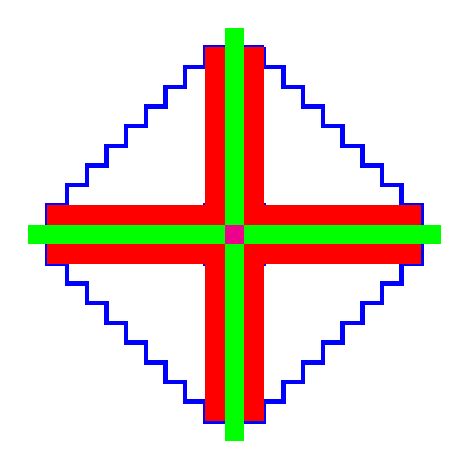
\begin{tikzpicture}[scale=0.25]
    

\draw [blue,ultra thick](2,10) -- (2,9) -- (3,9) -- (3,8) -- (4,8) -- (4,7) --  (5,7) node (v1) {} -- (5,6) -- (6,6) -- (6,5) -- (7,5) -- (7,4) -- (8,4) -- (8,3) -- (9,3) -- (9,2) -- (10,2) node (v2) {} -- (10,1) node (v10) {} -- (1,1) node (v3) {} -- (1,10) node (v9) {}--(2,10);
\draw [blue,ultra thick]  (2,2) rectangle (v3);

\draw [blue,ultra thick] (-9,0) -- (-9,-1) --(-8,-1)--(-8,-1) -- (-8,-2) -- (-7,-2) -- (-7,-3) -- (-6,-3) -- (-6,-4) --  (-5,-4) node (v1) {} -- (-5,-5) -- (-4,-5) -- (-4,-6) -- (-3,-6) -- (-3,-7) -- (-2,-7) -- (-2,-8) -- (-1,-8) -- (-1,-9) -- (0,-9) node (v2) {} -- (0,-9) node (v12) {} -- (0,0) node (v3) {} -- (-9,0) node (v11) {};
\draw [blue,ultra thick]  (-1,-1) rectangle (v3);
\draw [blue,ultra thick] (0,10) node (v4) {} -- (-1,10) -- (-1,9) node (v7) {} -- (-2,9) -- (-2,8) -- (-3,8) -- (-3,7) -- (-4,7) -- (-4,6) -- (-5,6) -- (-5,5) -- (-6,5) -- (-6,4) -- (-7,4) -- (-7,3) -- (-8,3) -- (-8,2) -- (-9,2) -- (-9,1) node (v8) {} -- (0,1) node (v5) {} -- (v4);
\draw [blue,ultra thick] (-1,2) rectangle (v5);
\draw [blue,ultra thick] (10,0) --(1,0) node (v6) {} -- (1,-9) -- (2,-9) -- (2,-8) -- (3,-8) -- (3,-7) -- (4,-7) -- (4,-6) -- (5,-6) -- (5,-5) -- (6,-5) -- (6,-4) -- (7,-4) -- (7,-3) -- (8,-3) -- (8,-2) -- (9,-2) -- (9,-1) -- (10,-1) node (v14) {} -- cycle;
\draw [blue,ultra thick] (v6) rectangle (2,-1);


\fill[red,ultra thick]  (-1,10) rectangle (0,1);
\fill[red,ultra thick]  (0,2) rectangle (v8);
\fill[red,ultra thick]  (v9) rectangle (2,1);
\fill[red,ultra thick]  (1,2) rectangle (v10);
\fill[red,ultra thick]  (v11) rectangle (0,-1);
\fill[red,ultra thick]  (-1,0) rectangle (v12);
\fill[red,ultra thick]  (v6) node (v13) {} rectangle (2,-9);
\fill[red,ultra thick]  (v13) rectangle (v14);


\fill[green,ultra thick]  (-10,1) rectangle (v3);
\fill[green,ultra thick]  (0,11) rectangle (1,1);
\fill[green,ultra thick]  (11,1) rectangle (1,0);
\fill[green,ultra thick]  (v3) rectangle (1,-10);
\fill[magenta]  (v5) rectangle (v6);

  \end{tikzpicture}
\end{center}
\begin{algorithm}[H]
\caption{STABLE for cases 12, 123, 124.}
\begin{algorithmic} 
% \REQUIRE Finite configuration in a square of $n\times n$.   % input
\STATE{ Find the smallest {{\bf \color{blue} blue}} square containing cells in state 1 in its boundary.}
  % \IF{not exists {{\color{blue} blue}}  square}
      % \RETURN {no change}
  % \ENDIF  
\STATE{ Compute {{\bf \color{red}red}} cells}  
\STATE{ Compute {{\bf \color{green}green}} cells}  
% \STATE{ Compute {{\color{magenta} center}}  cell}
\ENSURE Value in the {{\bf \color{magenta} center}} cell.          % output
\end{algorithmic}
\end{algorithm}
 }  
%%%%%%%%%%%%%%%%%%%%%%%%%%%%%%%%%%%%%%%%%%%%%%%%%%%%%%%%%%%%%%%%%%%%%%%%%%%%%%%%%%%%%%%%%%%%%%%%%%%%%%%%%%%%%%%%%%%%%%%%%%%%%%%%%%%%%%%%%%%%%%%%%%%%%%%%%%%%
  \headerbox{Complexity}{name=complex,column=2,span=2,row=3,below=ex}{
%%%%%%%%%%%%%%%%%%%%%%%%%%%%%%%%%%%%%%%%%%%%%%%%%%%%%%%%%%%%%%%%%%%%%%%%%%%%%%%%%%%%%%%%%%%%%%%%%%%%%%%%%%%%%%%%%%%%%%%%%%%%%%%%%%%%%%%%%%%%%%%%%%%%%%%%%%%%
\hspace*{-19pt}
{ \small
\begin{minipage}[t]{0.35\textwidth}
$\begin{array}{|c|c|}
  %{|c|>{\centering}p{30pt}|>{\centering}p{30pt}|>{\centering}p{30pt}|>{\centering}p{30pt}|c|}
  \hline
  F      &  { STABLE} \\   
  \hline   %&      &
  %T                &  \mathcal{O}(1)         \\
  4                &  \mathcal{O}(1)      \\
  3                &  \text{in NC}        \\
  34               &  \text{in NC}        \\
  2                &  \text{P-Complete}   \\
  24               &  \text{P-Complete}   \\
  23               &  \text{?}            \\
  234              &  \text{in NC}        \\
  1                &  \text{?}            \\
  14               &  \text{?}            \\
  13               &  \text{?}            \\
  134              &  \text{?}            \\
  12               &  \text{in NC}        \\
  124              &  \text{in NC}        \\
  123              &  \text{in NC}        \\
  1234             &  \text{in NC}        \\   
   \hline
  \end{array}$
\end{minipage}}  
\hspace{15pt}
\begin{minipage}[h]{0.525\textwidth}

\textbullet A {{\bf \color{red} stable cell}} (SC) is a cell that never changes.

\textbullet Decision problem  {{\bf \color{red}  STABLE}}:

{\bf Inputs:} TFCA $F$ and $c\in \{0,1\}^{\mathbb{Z}^2}$ a finite configuration. \\
{\bf Question:} \\Is $(0,0)$ a SC?         

\textbullet {\bf  \color{red} P}:  Problems solvable in polynomial time in a sequential machine.

\textbullet {\bf  \color{red} NC}: Problems solvable in poly-log   time in a parallel   machine.

\end{minipage} 
 }   
%%%%%%%%%%%%%%%%%%%%%%%%%%%%%%%%%%%%%%%%%%%%%%%%%%%%%%%%%%%%%%%%%%%%%%%%%%%%%%%%%%%%%%%%%%%%%%%%%%%%%%%%%%%%%%%%%%%%%%%%%%%%%%%%%%%%%%%%%%%%%%%%%%%%%%%%%%%%
  \headerbox{Case 234}{name=rule234,column=4,span=2,row=3,below=ex}{
%%%%%%%%%%%%%%%%%%%%%%%%%%%%%%%%%%%%%%%%%%%%%%%%%%%%%%%%%%%%%%%%%%%%%%%%%%%%%%%%%%%%%%%%%%%%%%%%%%%%%%%%%%%%%%%%%%%%%%%%%%%%%%%%%%%%%%%%%%%%%%%%%%%%%%%%%%%%

\begin{center}
  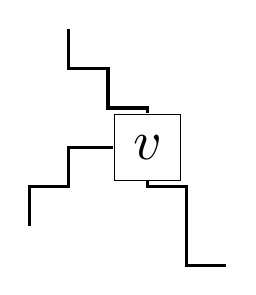
\begin{tikzpicture}[scale=1, every node/.style={scale=2.0}]]
\node (v1) at (-1.5,0)[draw,square] {$v$};
\draw[very thick] (v1) -- (-1.5,0.5) -- (-2,0.5) -- (-2,1) -- (-2.5,1) -- (-2.5,1.5);
\draw[very thick] (v1) -- (-2.5,0) -- (-2.5,-0.5) -- (-3,-0.5) -- (-3,-1);
\draw[very thick] (v1) -- (-1.5,-0.5) -- (-1,-0.5) -- (-1,-1.5) -- (-0.5,-1.5);
\end{tikzpicture}
\end{center}

A stable cell (SC) has 3 stable neighbors in state 0, then has 3 paths to the border.
\begin{center}
  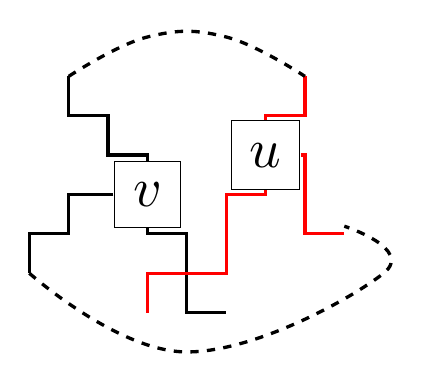
\begin{tikzpicture}[scale=1, every node/.style={scale=2.0}]]
\node (v1) at (-1.5,0)[draw,square] {$v$};
\draw[very thick] (v1) -- (-1.5,0.5) -- (-2,0.5) -- (-2,1) -- (-2.5,1) -- (-2.5,1.5);
\draw[very thick] (v1) -- (-2.5,0) -- (-2.5,-0.5) -- (-3,-0.5) -- (-3,-1);
\draw[very thick] (v1) -- (-1.5,-0.5) -- (-1,-0.5) -- (-1,-1.5) -- (-0.5,-1.5);
\node (v2) at (0,0.5)[draw,square] {$u$};
\draw[red,very thick] (v2) -- (0,1) -- (0.5,1) -- (0.5,1.5);
\draw[red,very thick] (v2) -- (0.5,0.5) -- (0.5,-0.5) -- (1,-0.5);
\draw[red,very thick] (v2) -- (0,0) -- (-0.5,0) -- (-0.5,-1) -- (-1.5,-1) -- (-1.5,-1.5);
\draw[dashed,very thick]  plot[smooth, tension=.7] coordinates {(-2.5,1.5) (-1.5,2) (-0.5,2) (0.5,1.5)};
\draw[dashed,very thick]  plot[smooth, tension=.7] coordinates {(-3,-1) (-1,-2) (1.5,-1) (1,-0.4029)};
\end{tikzpicture}
\end{center}

A pair of SC have 3 paths joining them, then they are a triply connected component (TCC) (computable in {\bf NC}).
\begin{algorithm}[H]
\caption{STABLE for case 234.}
\begin{algorithmic} 
% \REQUIRE Finite configuration in a square of $n\times n$.   % input
\STATE{ Find tri-connected components in the graph induced by cells initially in state 0.}
  \IF{$(0,0)$  is in a TCºC component }
    \RETURN {no change}
  \ELSE
    \RETURN {change}
  \ENDIF  
\end{algorithmic}
\end{algorithm}
 } 



%%%%%%%%%%%%%%%%%%%%%%%%%%%%%%%%%%%%%%%%%%%%%%%%%%%%%%%%%%%%%%%%%%%%%%%%%%%%%%%%%%%%%%%%%%%%%%%%%%%%%%%%%%%%%%%%%%%%%%%%%%%%%%%%%%%%%%%%%%%%%%%%%%%%%%%%%%%%
  \headerbox{Cases 2, 24}{name=rule2,column=2,span=2,row=4,below=complex}{
%%%%%%%%%%%%%%%%%%%%%%%%%%%%%%%%%%%%%%%%%%%%%%%%%%%%%%%%%%%%%%%%%%%%%%%%%%%%%%%%%%%%%%%%%%%%%%%%%%%%%%%%%%%%%%%%%%%%%%%%%%%%%%%%%%%%%%%%%%%%%%%%%%%%%%%%%%%%
\begin{center}
  \begin{minipage}[t]{0.325\textwidth}
      \begin{center} 
        \begin{tikzpicture}[scale=0.075]
          % Para incluir wire61_1.tex en un doc LaTeX se puede insertar el siguiente codigo:

% \usepackage{tikz}
% \usepackage{pgffor}
% 
% \foreach \n in {1,...,61}{
% \only<\n>{
% \begin{center} 
% 	\begin{tikzpicture}[scale=1.0]
% 		\input{./wire61/wire61_\n}
% 	\end{tikzpicture}
% \end{center}}}


\draw[color=gray, thick] (1,1) grid (29,29);
\draw[color=black, thick] (1,1) rectangle (29,29);
\fill[black] (1,23) rectangle (2,24); 
\fill[black] (2,23) rectangle (3,24); 
\fill[black] (3,23) rectangle (4,24); 
\fill[black] (4,23) rectangle (5,24); 
\fill[black] (5,23) rectangle (6,24); 
\fill[black] (6,23) rectangle (7,24); 
\fill[black] (7,23) rectangle (8,24); 
\fill[black] (8,23) rectangle (9,24); 
\fill[black] (9,23) rectangle (10,24); 
\fill[black] (24,23) rectangle (25,24); 
\fill[black] (25,23) rectangle (26,24); 
\fill[black] (26,23) rectangle (27,24); 
\fill[black] (27,23) rectangle (28,24); 
\fill[black] (28,23) rectangle (29,24); 
\fill[black] (1,22) rectangle (2,23); 
\fill[black] (2,22) rectangle (3,23); 
\fill[black] (3,22) rectangle (4,23); 
\fill[black] (4,22) rectangle (5,23); 
\fill[black] (5,22) rectangle (6,23); 
\fill[black] (6,22) rectangle (7,23); 
\fill[black] (7,22) rectangle (8,23); 
\fill[black] (8,22) rectangle (9,23); 
\fill[black] (9,22) rectangle (10,23); 
\fill[black] (21,22) rectangle (22,23); 
\fill[black] (24,22) rectangle (25,23); 
\fill[black] (25,22) rectangle (26,23); 
\fill[black] (26,22) rectangle (27,23); 
\fill[black] (27,22) rectangle (28,23); 
\fill[black] (28,22) rectangle (29,23); 
\fill[black] (1,21) rectangle (2,22); 
\fill[black] (11,21) rectangle (12,22); 
\fill[black] (12,21) rectangle (13,22); 
\fill[black] (11,20) rectangle (12,21); 
\fill[black] (12,20) rectangle (13,21); 
\fill[black] (22,20) rectangle (23,21); 
\fill[black] (23,20) rectangle (24,21); 
\fill[black] (11,19) rectangle (12,20); 
\fill[black] (12,19) rectangle (13,20); 
\fill[black] (22,19) rectangle (23,20); 
\fill[black] (23,19) rectangle (24,20); 
\fill[black] (25,19) rectangle (26,20); 
\fill[black] (8,18) rectangle (9,19); 
\fill[black] (11,18) rectangle (12,19); 
\fill[black] (12,18) rectangle (13,19); 
\fill[black] (22,18) rectangle (23,19); 
\fill[black] (23,18) rectangle (24,19); 
\fill[black] (24,18) rectangle (25,19); 
\fill[black] (11,17) rectangle (12,18); 
\fill[black] (12,17) rectangle (13,18); 
\fill[black] (22,17) rectangle (23,18); 
\fill[black] (23,17) rectangle (24,18); 
\fill[black] (25,17) rectangle (26,18); 
\fill[black] (11,16) rectangle (12,17); 
\fill[black] (12,16) rectangle (13,17); 
\fill[black] (22,16) rectangle (23,17); 
\fill[black] (23,16) rectangle (24,17); 
\fill[black] (11,15) rectangle (12,16); 
\fill[black] (12,15) rectangle (13,16); 
\fill[black] (22,15) rectangle (23,16); 
\fill[black] (23,15) rectangle (24,16); 
\fill[black] (11,14) rectangle (12,15); 
\fill[black] (12,14) rectangle (13,15); 
\fill[black] (22,14) rectangle (23,15); 
\fill[black] (23,14) rectangle (24,15); 
\fill[black] (11,13) rectangle (12,14); 
\fill[black] (12,13) rectangle (13,14); 
\fill[black] (22,13) rectangle (23,14); 
\fill[black] (23,13) rectangle (24,14); 
\fill[black] (11,12) rectangle (12,13); 
\fill[black] (12,12) rectangle (13,13); 
\fill[black] (22,12) rectangle (23,13); 
\fill[black] (23,12) rectangle (24,13); 
\fill[black] (11,11) rectangle (12,12); 
\fill[black] (12,11) rectangle (13,12); 
\fill[black] (22,11) rectangle (23,12); 
\fill[black] (23,11) rectangle (24,12); 
\fill[black] (11,10) rectangle (12,11); 
\fill[black] (12,10) rectangle (13,11); 
\fill[black] (22,10) rectangle (23,11); 
\fill[black] (23,10) rectangle (24,11); 
\fill[black] (11,9) rectangle (12,10); 
\fill[black] (12,9) rectangle (13,10); 
\fill[black] (22,9) rectangle (23,10); 
\fill[black] (23,9) rectangle (24,10); 
\fill[black] (11,8) rectangle (12,9); 
\fill[black] (12,8) rectangle (13,9); 
\fill[black] (14,8) rectangle (15,9); 
\fill[black] (17,8) rectangle (18,9); 
\fill[black] (19,8) rectangle (20,9); 
\fill[black] (22,8) rectangle (23,9); 
\fill[black] (23,8) rectangle (24,9); 
\fill[black] (11,7) rectangle (12,8); 
\fill[black] (12,7) rectangle (13,8); 
\fill[black] (13,7) rectangle (14,8); 
\fill[black] (18,7) rectangle (19,8); 
\fill[black] (22,7) rectangle (23,8); 
\fill[black] (23,7) rectangle (24,8); 
\fill[black] (11,6) rectangle (12,7); 
\fill[black] (12,6) rectangle (13,7); 
\fill[black] (13,6) rectangle (14,7); 
\fill[black] (14,6) rectangle (15,7); 
\fill[black] (15,6) rectangle (16,7); 
\fill[black] (16,6) rectangle (17,7); 
\fill[black] (17,6) rectangle (18,7); 
\fill[black] (18,6) rectangle (19,7); 
\fill[black] (19,6) rectangle (20,7); 
\fill[black] (20,6) rectangle (21,7); 
\fill[black] (11,5) rectangle (12,6); 
\fill[black] (12,5) rectangle (13,6); 
\fill[black] (13,5) rectangle (14,6); 
\fill[black] (14,5) rectangle (15,6); 
\fill[black] (15,5) rectangle (16,6); 
\fill[black] (16,5) rectangle (17,6); 
\fill[black] (17,5) rectangle (18,6); 
\fill[black] (18,5) rectangle (19,6); 
\fill[black] (19,5) rectangle (20,6); 
\fill[black] (20,5) rectangle (21,6); 
\fill[black] (22,4) rectangle (23,5); 
\fill[black] (23,4) rectangle (24,5); 
\fill[black] (10,3) rectangle (11,4); 
\fill[black] (12,2) rectangle (13,3); 

        \end{tikzpicture}\\
      Wire
      \end{center}  
  \end{minipage}            
  \begin{minipage}[t]{0.325\textwidth}
      \begin{center}
      \begin{tikzpicture}[scale=0.075]
        \draw[color=gray, thick] (1,1) grid (29,29);
\draw[color=black, thick] (1,1) rectangle (29,29);

% Para incluir x2.tex en un doc LaTeX se puede insertar el siguiente codigo:
% \begin{tikzpicture}[scale=1.0]
% 	\draw[color=gray, thick] (1,1) grid (29,29);
\draw[color=black, thick] (1,1) rectangle (29,29);

% Para incluir x2.tex en un doc LaTeX se puede insertar el siguiente codigo:
% \begin{tikzpicture}[scale=1.0]
% 	\draw[color=gray, thick] (1,1) grid (29,29);
\draw[color=black, thick] (1,1) rectangle (29,29);

% Para incluir x2.tex en un doc LaTeX se puede insertar el siguiente codigo:
% \begin{tikzpicture}[scale=1.0]
% 	\input{./x2}
% \end{tikzpicture}
\fill[black] (15,26) rectangle (16,27); 
\fill[black] (16,26) rectangle (17,27); 
\fill[black] (17,26) rectangle (18,27); 
\fill[black] (18,26) rectangle (19,27); 
\fill[black] (19,26) rectangle (20,27); 
\fill[black] (20,26) rectangle (21,27); 
\fill[black] (21,26) rectangle (22,27); 
\fill[black] (22,26) rectangle (23,27); 
\fill[black] (23,26) rectangle (24,27); 
\fill[black] (24,26) rectangle (25,27); 
\fill[black] (25,26) rectangle (26,27); 
\fill[black] (26,26) rectangle (27,27); 
\fill[black] (27,26) rectangle (28,27); 
\fill[black] (28,26) rectangle (29,27); 
\fill[black] (12,25) rectangle (13,26); 
\fill[black] (15,25) rectangle (16,26); 
\fill[black] (16,25) rectangle (17,26); 
\fill[black] (17,25) rectangle (18,26); 
\fill[black] (18,25) rectangle (19,26); 
\fill[black] (19,25) rectangle (20,26); 
\fill[black] (20,25) rectangle (21,26); 
\fill[black] (21,25) rectangle (22,26); 
\fill[black] (22,25) rectangle (23,26); 
\fill[black] (23,25) rectangle (24,26); 
\fill[black] (24,25) rectangle (25,26); 
\fill[black] (25,25) rectangle (26,26); 
\fill[black] (26,25) rectangle (27,26); 
\fill[black] (27,25) rectangle (28,26); 
\fill[black] (28,25) rectangle (29,26); 
\fill[black] (13,23) rectangle (14,24); 
\fill[black] (13,22) rectangle (14,23); 
\fill[black] (16,22) rectangle (17,23); 
\fill[black] (13,21) rectangle (14,22); 
\fill[black] (13,20) rectangle (14,21); 
\fill[black] (13,19) rectangle (14,20); 
\fill[black] (13,18) rectangle (14,19); 
\fill[black] (13,17) rectangle (14,18); 
\fill[black] (13,16) rectangle (14,17); 
\fill[black] (1,15) rectangle (2,16); 
\fill[black] (2,15) rectangle (3,16); 
\fill[black] (3,15) rectangle (4,16); 
\fill[black] (4,15) rectangle (5,16); 
\fill[black] (5,15) rectangle (6,16); 
\fill[black] (6,15) rectangle (7,16); 
\fill[black] (7,15) rectangle (8,16); 
\fill[black] (8,15) rectangle (9,16); 
\fill[black] (9,15) rectangle (10,16); 
\fill[black] (10,15) rectangle (11,16); 
\fill[black] (11,15) rectangle (12,16); 
\fill[black] (1,14) rectangle (2,15); 
\fill[black] (2,14) rectangle (3,15); 
\fill[black] (3,14) rectangle (4,15); 
\fill[black] (4,14) rectangle (5,15); 
\fill[black] (5,14) rectangle (6,15); 
\fill[black] (6,14) rectangle (7,15); 
\fill[black] (7,14) rectangle (8,15); 
\fill[black] (8,14) rectangle (9,15); 
\fill[black] (9,14) rectangle (10,15); 
\fill[black] (10,14) rectangle (11,15); 
\fill[black] (11,14) rectangle (12,15); 
\fill[black] (1,13) rectangle (2,14); 
\fill[black] (13,13) rectangle (14,14); 
\fill[black] (14,13) rectangle (15,14); 
\fill[black] (13,12) rectangle (14,13); 
\fill[black] (14,12) rectangle (15,13); 
\fill[black] (13,11) rectangle (14,12); 
\fill[black] (14,11) rectangle (15,12); 
\fill[black] (10,10) rectangle (11,11); 
\fill[black] (13,10) rectangle (14,11); 
\fill[black] (14,10) rectangle (15,11); 
\fill[black] (13,9) rectangle (14,10); 
\fill[black] (14,9) rectangle (15,10); 
\fill[black] (16,9) rectangle (17,10); 
\fill[black] (17,9) rectangle (18,10); 
\fill[black] (13,8) rectangle (14,9); 
\fill[black] (14,8) rectangle (15,9); 
\fill[black] (15,8) rectangle (16,9); 
\fill[black] (17,8) rectangle (18,9); 
\fill[black] (13,7) rectangle (14,8); 
\fill[black] (14,7) rectangle (15,8); 
\fill[black] (15,7) rectangle (16,8); 
\fill[black] (13,6) rectangle (14,7); 
\fill[black] (14,6) rectangle (15,7); 
\fill[black] (15,6) rectangle (16,7); 
\fill[black] (13,5) rectangle (14,6); 
\fill[black] (14,5) rectangle (15,6); 
\fill[black] (15,5) rectangle (16,6); 
\fill[black] (18,5) rectangle (19,6); 
\fill[black] (19,5) rectangle (20,6); 
\fill[black] (13,4) rectangle (14,5); 
\fill[black] (14,4) rectangle (15,5); 
\fill[black] (15,4) rectangle (16,5); 
\fill[black] (18,4) rectangle (19,5); 
\fill[black] (19,4) rectangle (20,5); 
\fill[black] (22,4) rectangle (23,5); 
\fill[black] (23,4) rectangle (24,5); 
\fill[black] (24,4) rectangle (25,5); 
\fill[black] (25,4) rectangle (26,5); 
\fill[black] (26,4) rectangle (27,5); 
\fill[black] (27,4) rectangle (28,5); 
\fill[black] (28,4) rectangle (29,5); 
\fill[black] (11,3) rectangle (12,4); 
\fill[black] (22,3) rectangle (23,4); 
\fill[black] (23,3) rectangle (24,4); 
\fill[black] (24,3) rectangle (25,4); 
\fill[black] (25,3) rectangle (26,4); 
\fill[black] (26,3) rectangle (27,4); 
\fill[black] (27,3) rectangle (28,4); 
\fill[black] (28,3) rectangle (29,4); 
\fill[black] (16,2) rectangle (17,3); 
\fill[black] (20,2) rectangle (21,3); 
% \end{tikzpicture}
\fill[black] (15,26) rectangle (16,27); 
\fill[black] (16,26) rectangle (17,27); 
\fill[black] (17,26) rectangle (18,27); 
\fill[black] (18,26) rectangle (19,27); 
\fill[black] (19,26) rectangle (20,27); 
\fill[black] (20,26) rectangle (21,27); 
\fill[black] (21,26) rectangle (22,27); 
\fill[black] (22,26) rectangle (23,27); 
\fill[black] (23,26) rectangle (24,27); 
\fill[black] (24,26) rectangle (25,27); 
\fill[black] (25,26) rectangle (26,27); 
\fill[black] (26,26) rectangle (27,27); 
\fill[black] (27,26) rectangle (28,27); 
\fill[black] (28,26) rectangle (29,27); 
\fill[black] (12,25) rectangle (13,26); 
\fill[black] (15,25) rectangle (16,26); 
\fill[black] (16,25) rectangle (17,26); 
\fill[black] (17,25) rectangle (18,26); 
\fill[black] (18,25) rectangle (19,26); 
\fill[black] (19,25) rectangle (20,26); 
\fill[black] (20,25) rectangle (21,26); 
\fill[black] (21,25) rectangle (22,26); 
\fill[black] (22,25) rectangle (23,26); 
\fill[black] (23,25) rectangle (24,26); 
\fill[black] (24,25) rectangle (25,26); 
\fill[black] (25,25) rectangle (26,26); 
\fill[black] (26,25) rectangle (27,26); 
\fill[black] (27,25) rectangle (28,26); 
\fill[black] (28,25) rectangle (29,26); 
\fill[black] (13,23) rectangle (14,24); 
\fill[black] (13,22) rectangle (14,23); 
\fill[black] (16,22) rectangle (17,23); 
\fill[black] (13,21) rectangle (14,22); 
\fill[black] (13,20) rectangle (14,21); 
\fill[black] (13,19) rectangle (14,20); 
\fill[black] (13,18) rectangle (14,19); 
\fill[black] (13,17) rectangle (14,18); 
\fill[black] (13,16) rectangle (14,17); 
\fill[black] (1,15) rectangle (2,16); 
\fill[black] (2,15) rectangle (3,16); 
\fill[black] (3,15) rectangle (4,16); 
\fill[black] (4,15) rectangle (5,16); 
\fill[black] (5,15) rectangle (6,16); 
\fill[black] (6,15) rectangle (7,16); 
\fill[black] (7,15) rectangle (8,16); 
\fill[black] (8,15) rectangle (9,16); 
\fill[black] (9,15) rectangle (10,16); 
\fill[black] (10,15) rectangle (11,16); 
\fill[black] (11,15) rectangle (12,16); 
\fill[black] (1,14) rectangle (2,15); 
\fill[black] (2,14) rectangle (3,15); 
\fill[black] (3,14) rectangle (4,15); 
\fill[black] (4,14) rectangle (5,15); 
\fill[black] (5,14) rectangle (6,15); 
\fill[black] (6,14) rectangle (7,15); 
\fill[black] (7,14) rectangle (8,15); 
\fill[black] (8,14) rectangle (9,15); 
\fill[black] (9,14) rectangle (10,15); 
\fill[black] (10,14) rectangle (11,15); 
\fill[black] (11,14) rectangle (12,15); 
\fill[black] (1,13) rectangle (2,14); 
\fill[black] (13,13) rectangle (14,14); 
\fill[black] (14,13) rectangle (15,14); 
\fill[black] (13,12) rectangle (14,13); 
\fill[black] (14,12) rectangle (15,13); 
\fill[black] (13,11) rectangle (14,12); 
\fill[black] (14,11) rectangle (15,12); 
\fill[black] (10,10) rectangle (11,11); 
\fill[black] (13,10) rectangle (14,11); 
\fill[black] (14,10) rectangle (15,11); 
\fill[black] (13,9) rectangle (14,10); 
\fill[black] (14,9) rectangle (15,10); 
\fill[black] (16,9) rectangle (17,10); 
\fill[black] (17,9) rectangle (18,10); 
\fill[black] (13,8) rectangle (14,9); 
\fill[black] (14,8) rectangle (15,9); 
\fill[black] (15,8) rectangle (16,9); 
\fill[black] (17,8) rectangle (18,9); 
\fill[black] (13,7) rectangle (14,8); 
\fill[black] (14,7) rectangle (15,8); 
\fill[black] (15,7) rectangle (16,8); 
\fill[black] (13,6) rectangle (14,7); 
\fill[black] (14,6) rectangle (15,7); 
\fill[black] (15,6) rectangle (16,7); 
\fill[black] (13,5) rectangle (14,6); 
\fill[black] (14,5) rectangle (15,6); 
\fill[black] (15,5) rectangle (16,6); 
\fill[black] (18,5) rectangle (19,6); 
\fill[black] (19,5) rectangle (20,6); 
\fill[black] (13,4) rectangle (14,5); 
\fill[black] (14,4) rectangle (15,5); 
\fill[black] (15,4) rectangle (16,5); 
\fill[black] (18,4) rectangle (19,5); 
\fill[black] (19,4) rectangle (20,5); 
\fill[black] (22,4) rectangle (23,5); 
\fill[black] (23,4) rectangle (24,5); 
\fill[black] (24,4) rectangle (25,5); 
\fill[black] (25,4) rectangle (26,5); 
\fill[black] (26,4) rectangle (27,5); 
\fill[black] (27,4) rectangle (28,5); 
\fill[black] (28,4) rectangle (29,5); 
\fill[black] (11,3) rectangle (12,4); 
\fill[black] (22,3) rectangle (23,4); 
\fill[black] (23,3) rectangle (24,4); 
\fill[black] (24,3) rectangle (25,4); 
\fill[black] (25,3) rectangle (26,4); 
\fill[black] (26,3) rectangle (27,4); 
\fill[black] (27,3) rectangle (28,4); 
\fill[black] (28,3) rectangle (29,4); 
\fill[black] (16,2) rectangle (17,3); 
\fill[black] (20,2) rectangle (21,3); 
% \end{tikzpicture}
\fill[black] (15,26) rectangle (16,27); 
\fill[black] (16,26) rectangle (17,27); 
\fill[black] (17,26) rectangle (18,27); 
\fill[black] (18,26) rectangle (19,27); 
\fill[black] (19,26) rectangle (20,27); 
\fill[black] (20,26) rectangle (21,27); 
\fill[black] (21,26) rectangle (22,27); 
\fill[black] (22,26) rectangle (23,27); 
\fill[black] (23,26) rectangle (24,27); 
\fill[black] (24,26) rectangle (25,27); 
\fill[black] (25,26) rectangle (26,27); 
\fill[black] (26,26) rectangle (27,27); 
\fill[black] (27,26) rectangle (28,27); 
\fill[black] (28,26) rectangle (29,27); 
\fill[black] (12,25) rectangle (13,26); 
\fill[black] (15,25) rectangle (16,26); 
\fill[black] (16,25) rectangle (17,26); 
\fill[black] (17,25) rectangle (18,26); 
\fill[black] (18,25) rectangle (19,26); 
\fill[black] (19,25) rectangle (20,26); 
\fill[black] (20,25) rectangle (21,26); 
\fill[black] (21,25) rectangle (22,26); 
\fill[black] (22,25) rectangle (23,26); 
\fill[black] (23,25) rectangle (24,26); 
\fill[black] (24,25) rectangle (25,26); 
\fill[black] (25,25) rectangle (26,26); 
\fill[black] (26,25) rectangle (27,26); 
\fill[black] (27,25) rectangle (28,26); 
\fill[black] (28,25) rectangle (29,26); 
\fill[black] (13,23) rectangle (14,24); 
\fill[black] (13,22) rectangle (14,23); 
\fill[black] (16,22) rectangle (17,23); 
\fill[black] (13,21) rectangle (14,22); 
\fill[black] (13,20) rectangle (14,21); 
\fill[black] (13,19) rectangle (14,20); 
\fill[black] (13,18) rectangle (14,19); 
\fill[black] (13,17) rectangle (14,18); 
\fill[black] (13,16) rectangle (14,17); 
\fill[black] (1,15) rectangle (2,16); 
\fill[black] (2,15) rectangle (3,16); 
\fill[black] (3,15) rectangle (4,16); 
\fill[black] (4,15) rectangle (5,16); 
\fill[black] (5,15) rectangle (6,16); 
\fill[black] (6,15) rectangle (7,16); 
\fill[black] (7,15) rectangle (8,16); 
\fill[black] (8,15) rectangle (9,16); 
\fill[black] (9,15) rectangle (10,16); 
\fill[black] (10,15) rectangle (11,16); 
\fill[black] (11,15) rectangle (12,16); 
\fill[black] (1,14) rectangle (2,15); 
\fill[black] (2,14) rectangle (3,15); 
\fill[black] (3,14) rectangle (4,15); 
\fill[black] (4,14) rectangle (5,15); 
\fill[black] (5,14) rectangle (6,15); 
\fill[black] (6,14) rectangle (7,15); 
\fill[black] (7,14) rectangle (8,15); 
\fill[black] (8,14) rectangle (9,15); 
\fill[black] (9,14) rectangle (10,15); 
\fill[black] (10,14) rectangle (11,15); 
\fill[black] (11,14) rectangle (12,15); 
\fill[black] (1,13) rectangle (2,14); 
\fill[black] (13,13) rectangle (14,14); 
\fill[black] (14,13) rectangle (15,14); 
\fill[black] (13,12) rectangle (14,13); 
\fill[black] (14,12) rectangle (15,13); 
\fill[black] (13,11) rectangle (14,12); 
\fill[black] (14,11) rectangle (15,12); 
\fill[black] (10,10) rectangle (11,11); 
\fill[black] (13,10) rectangle (14,11); 
\fill[black] (14,10) rectangle (15,11); 
\fill[black] (13,9) rectangle (14,10); 
\fill[black] (14,9) rectangle (15,10); 
\fill[black] (16,9) rectangle (17,10); 
\fill[black] (17,9) rectangle (18,10); 
\fill[black] (13,8) rectangle (14,9); 
\fill[black] (14,8) rectangle (15,9); 
\fill[black] (15,8) rectangle (16,9); 
\fill[black] (17,8) rectangle (18,9); 
\fill[black] (13,7) rectangle (14,8); 
\fill[black] (14,7) rectangle (15,8); 
\fill[black] (15,7) rectangle (16,8); 
\fill[black] (13,6) rectangle (14,7); 
\fill[black] (14,6) rectangle (15,7); 
\fill[black] (15,6) rectangle (16,7); 
\fill[black] (13,5) rectangle (14,6); 
\fill[black] (14,5) rectangle (15,6); 
\fill[black] (15,5) rectangle (16,6); 
\fill[black] (18,5) rectangle (19,6); 
\fill[black] (19,5) rectangle (20,6); 
\fill[black] (13,4) rectangle (14,5); 
\fill[black] (14,4) rectangle (15,5); 
\fill[black] (15,4) rectangle (16,5); 
\fill[black] (18,4) rectangle (19,5); 
\fill[black] (19,4) rectangle (20,5); 
\fill[black] (22,4) rectangle (23,5); 
\fill[black] (23,4) rectangle (24,5); 
\fill[black] (24,4) rectangle (25,5); 
\fill[black] (25,4) rectangle (26,5); 
\fill[black] (26,4) rectangle (27,5); 
\fill[black] (27,4) rectangle (28,5); 
\fill[black] (28,4) rectangle (29,5); 
\fill[black] (11,3) rectangle (12,4); 
\fill[black] (22,3) rectangle (23,4); 
\fill[black] (23,3) rectangle (24,4); 
\fill[black] (24,3) rectangle (25,4); 
\fill[black] (25,3) rectangle (26,4); 
\fill[black] (26,3) rectangle (27,4); 
\fill[black] (27,3) rectangle (28,4); 
\fill[black] (28,3) rectangle (29,4); 
\fill[black] (16,2) rectangle (17,3); 
\fill[black] (20,2) rectangle (21,3);  % Seleccionar 28x28 celdas en golly
      \end{tikzpicture}\\
      Duplicator
      \end{center}
      \end{minipage}            

  \begin{minipage}[t]{0.325\textwidth}
      \begin{center}
      \begin{tikzpicture}[scale=0.075]
        \draw[color=gray, thick] (1,1) grid (29,29);
\draw[color=black, thick] (1,1) rectangle (29,29);

% Para incluir AND.tex en un doc LaTeX se puede insertar el siguiente codigo:
% \begin{tikzpicture}[scale=1.0]
% 	\draw[color=gray, thick] (1,1) grid (29,29);
\draw[color=black, thick] (1,1) rectangle (29,29);

% Para incluir AND.tex en un doc LaTeX se puede insertar el siguiente codigo:
% \begin{tikzpicture}[scale=1.0]
% 	\draw[color=gray, thick] (1,1) grid (29,29);
\draw[color=black, thick] (1,1) rectangle (29,29);

% Para incluir AND.tex en un doc LaTeX se puede insertar el siguiente codigo:
% \begin{tikzpicture}[scale=1.0]
% 	\input{./AND}
% \end{tikzpicture}
\fill[black] (1,27) rectangle (2,28); 
\fill[black] (2,27) rectangle (3,28); 
\fill[black] (3,27) rectangle (4,28); 
\fill[black] (4,27) rectangle (5,28); 
\fill[black] (5,27) rectangle (6,28); 
\fill[black] (6,27) rectangle (7,28); 
\fill[black] (7,27) rectangle (8,28); 
\fill[black] (1,26) rectangle (2,27); 
\fill[black] (2,26) rectangle (3,27); 
\fill[black] (3,26) rectangle (4,27); 
\fill[black] (4,26) rectangle (5,27); 
\fill[black] (5,26) rectangle (6,27); 
\fill[black] (6,26) rectangle (7,27); 
\fill[black] (7,26) rectangle (8,27); 
\fill[black] (1,25) rectangle (2,26); 
\fill[black] (8,24) rectangle (9,25); 
\fill[black] (5,23) rectangle (6,24); 
\fill[black] (6,23) rectangle (7,24); 
\fill[black] (5,22) rectangle (6,23); 
\fill[black] (6,22) rectangle (7,23); 
\fill[black] (5,21) rectangle (6,22); 
\fill[black] (6,21) rectangle (7,22); 
\fill[black] (5,20) rectangle (6,21); 
\fill[black] (6,20) rectangle (7,21); 
\fill[black] (10,20) rectangle (11,21); 
\fill[black] (5,19) rectangle (6,20); 
\fill[black] (6,19) rectangle (7,20); 
\fill[black] (3,18) rectangle (4,19); 
\fill[black] (5,18) rectangle (6,19); 
\fill[black] (6,18) rectangle (7,19); 
\fill[black] (13,18) rectangle (14,19); 
\fill[black] (14,18) rectangle (15,19); 
\fill[black] (17,18) rectangle (18,19); 
\fill[black] (18,18) rectangle (19,19); 
\fill[black] (3,17) rectangle (4,18); 
\fill[black] (4,17) rectangle (5,18); 
\fill[black] (6,17) rectangle (7,18); 
\fill[black] (14,17) rectangle (15,18); 
\fill[black] (17,17) rectangle (18,18); 
\fill[black] (6,16) rectangle (7,17); 
\fill[black] (12,16) rectangle (13,17); 
\fill[black] (13,16) rectangle (14,17); 
\fill[black] (18,16) rectangle (19,17); 
\fill[black] (19,16) rectangle (20,17); 
\fill[black] (22,16) rectangle (23,17); 
\fill[black] (23,16) rectangle (24,17); 
\fill[black] (24,16) rectangle (25,17); 
\fill[black] (25,16) rectangle (26,17); 
\fill[black] (26,16) rectangle (27,17); 
\fill[black] (27,16) rectangle (28,17); 
\fill[black] (28,16) rectangle (29,17); 
\fill[black] (6,15) rectangle (7,16); 
\fill[black] (12,15) rectangle (13,16); 
\fill[black] (13,15) rectangle (14,16); 
\fill[black] (14,15) rectangle (15,16); 
\fill[black] (15,15) rectangle (16,16); 
\fill[black] (16,15) rectangle (17,16); 
\fill[black] (17,15) rectangle (18,16); 
\fill[black] (18,15) rectangle (19,16); 
\fill[black] (19,15) rectangle (20,16); 
\fill[black] (22,15) rectangle (23,16); 
\fill[black] (23,15) rectangle (24,16); 
\fill[black] (24,15) rectangle (25,16); 
\fill[black] (25,15) rectangle (26,16); 
\fill[black] (26,15) rectangle (27,16); 
\fill[black] (27,15) rectangle (28,16); 
\fill[black] (28,15) rectangle (29,16); 
\fill[black] (8,13) rectangle (9,14); 
\fill[black] (9,13) rectangle (10,14); 
\fill[black] (21,13) rectangle (22,14); 
\fill[black] (8,12) rectangle (9,13); 
\fill[black] (9,12) rectangle (10,13); 
\fill[black] (16,12) rectangle (17,13); 
\fill[black] (19,12) rectangle (20,13); 
\fill[black] (24,12) rectangle (25,13); 
\fill[black] (8,11) rectangle (9,12); 
\fill[black] (9,11) rectangle (10,12); 
\fill[black] (14,11) rectangle (15,12); 
\fill[black] (8,10) rectangle (9,11); 
\fill[black] (9,10) rectangle (10,11); 
\fill[black] (8,9) rectangle (9,10); 
\fill[black] (9,9) rectangle (10,10); 
\fill[black] (5,8) rectangle (6,9); 
\fill[black] (6,8) rectangle (7,9); 
\fill[black] (8,8) rectangle (9,9); 
\fill[black] (9,8) rectangle (10,9); 
\fill[black] (5,7) rectangle (6,8); 
\fill[black] (6,7) rectangle (7,8); 
\fill[black] (7,7) rectangle (8,8); 
\fill[black] (8,7) rectangle (9,8); 
\fill[black] (9,7) rectangle (10,8); 
\fill[black] (6,6) rectangle (7,7); 
\fill[black] (7,6) rectangle (8,7); 
\fill[black] (8,6) rectangle (9,7); 
\fill[black] (9,6) rectangle (10,7); 
\fill[black] (1,5) rectangle (2,6); 
\fill[black] (2,5) rectangle (3,6); 
\fill[black] (3,5) rectangle (4,6); 
\fill[black] (4,5) rectangle (5,6); 
\fill[black] (5,5) rectangle (6,6); 
\fill[black] (6,5) rectangle (7,6); 
\fill[black] (7,5) rectangle (8,6); 
\fill[black] (8,5) rectangle (9,6); 
\fill[black] (9,5) rectangle (10,6); 
\fill[black] (1,4) rectangle (2,5); 
\fill[black] (2,4) rectangle (3,5); 
\fill[black] (3,4) rectangle (4,5); 
\fill[black] (4,4) rectangle (5,5); 
\fill[black] (5,4) rectangle (6,5); 
\fill[black] (6,4) rectangle (7,5); 
\fill[black] (7,4) rectangle (8,5); 
\fill[black] (8,4) rectangle (9,5); 
\fill[black] (9,4) rectangle (10,5); 
\fill[black] (1,3) rectangle (2,4); 
\fill[black] (11,3) rectangle (12,4); 
% \end{tikzpicture}
\fill[black] (1,27) rectangle (2,28); 
\fill[black] (2,27) rectangle (3,28); 
\fill[black] (3,27) rectangle (4,28); 
\fill[black] (4,27) rectangle (5,28); 
\fill[black] (5,27) rectangle (6,28); 
\fill[black] (6,27) rectangle (7,28); 
\fill[black] (7,27) rectangle (8,28); 
\fill[black] (1,26) rectangle (2,27); 
\fill[black] (2,26) rectangle (3,27); 
\fill[black] (3,26) rectangle (4,27); 
\fill[black] (4,26) rectangle (5,27); 
\fill[black] (5,26) rectangle (6,27); 
\fill[black] (6,26) rectangle (7,27); 
\fill[black] (7,26) rectangle (8,27); 
\fill[black] (1,25) rectangle (2,26); 
\fill[black] (8,24) rectangle (9,25); 
\fill[black] (5,23) rectangle (6,24); 
\fill[black] (6,23) rectangle (7,24); 
\fill[black] (5,22) rectangle (6,23); 
\fill[black] (6,22) rectangle (7,23); 
\fill[black] (5,21) rectangle (6,22); 
\fill[black] (6,21) rectangle (7,22); 
\fill[black] (5,20) rectangle (6,21); 
\fill[black] (6,20) rectangle (7,21); 
\fill[black] (10,20) rectangle (11,21); 
\fill[black] (5,19) rectangle (6,20); 
\fill[black] (6,19) rectangle (7,20); 
\fill[black] (3,18) rectangle (4,19); 
\fill[black] (5,18) rectangle (6,19); 
\fill[black] (6,18) rectangle (7,19); 
\fill[black] (13,18) rectangle (14,19); 
\fill[black] (14,18) rectangle (15,19); 
\fill[black] (17,18) rectangle (18,19); 
\fill[black] (18,18) rectangle (19,19); 
\fill[black] (3,17) rectangle (4,18); 
\fill[black] (4,17) rectangle (5,18); 
\fill[black] (6,17) rectangle (7,18); 
\fill[black] (14,17) rectangle (15,18); 
\fill[black] (17,17) rectangle (18,18); 
\fill[black] (6,16) rectangle (7,17); 
\fill[black] (12,16) rectangle (13,17); 
\fill[black] (13,16) rectangle (14,17); 
\fill[black] (18,16) rectangle (19,17); 
\fill[black] (19,16) rectangle (20,17); 
\fill[black] (22,16) rectangle (23,17); 
\fill[black] (23,16) rectangle (24,17); 
\fill[black] (24,16) rectangle (25,17); 
\fill[black] (25,16) rectangle (26,17); 
\fill[black] (26,16) rectangle (27,17); 
\fill[black] (27,16) rectangle (28,17); 
\fill[black] (28,16) rectangle (29,17); 
\fill[black] (6,15) rectangle (7,16); 
\fill[black] (12,15) rectangle (13,16); 
\fill[black] (13,15) rectangle (14,16); 
\fill[black] (14,15) rectangle (15,16); 
\fill[black] (15,15) rectangle (16,16); 
\fill[black] (16,15) rectangle (17,16); 
\fill[black] (17,15) rectangle (18,16); 
\fill[black] (18,15) rectangle (19,16); 
\fill[black] (19,15) rectangle (20,16); 
\fill[black] (22,15) rectangle (23,16); 
\fill[black] (23,15) rectangle (24,16); 
\fill[black] (24,15) rectangle (25,16); 
\fill[black] (25,15) rectangle (26,16); 
\fill[black] (26,15) rectangle (27,16); 
\fill[black] (27,15) rectangle (28,16); 
\fill[black] (28,15) rectangle (29,16); 
\fill[black] (8,13) rectangle (9,14); 
\fill[black] (9,13) rectangle (10,14); 
\fill[black] (21,13) rectangle (22,14); 
\fill[black] (8,12) rectangle (9,13); 
\fill[black] (9,12) rectangle (10,13); 
\fill[black] (16,12) rectangle (17,13); 
\fill[black] (19,12) rectangle (20,13); 
\fill[black] (24,12) rectangle (25,13); 
\fill[black] (8,11) rectangle (9,12); 
\fill[black] (9,11) rectangle (10,12); 
\fill[black] (14,11) rectangle (15,12); 
\fill[black] (8,10) rectangle (9,11); 
\fill[black] (9,10) rectangle (10,11); 
\fill[black] (8,9) rectangle (9,10); 
\fill[black] (9,9) rectangle (10,10); 
\fill[black] (5,8) rectangle (6,9); 
\fill[black] (6,8) rectangle (7,9); 
\fill[black] (8,8) rectangle (9,9); 
\fill[black] (9,8) rectangle (10,9); 
\fill[black] (5,7) rectangle (6,8); 
\fill[black] (6,7) rectangle (7,8); 
\fill[black] (7,7) rectangle (8,8); 
\fill[black] (8,7) rectangle (9,8); 
\fill[black] (9,7) rectangle (10,8); 
\fill[black] (6,6) rectangle (7,7); 
\fill[black] (7,6) rectangle (8,7); 
\fill[black] (8,6) rectangle (9,7); 
\fill[black] (9,6) rectangle (10,7); 
\fill[black] (1,5) rectangle (2,6); 
\fill[black] (2,5) rectangle (3,6); 
\fill[black] (3,5) rectangle (4,6); 
\fill[black] (4,5) rectangle (5,6); 
\fill[black] (5,5) rectangle (6,6); 
\fill[black] (6,5) rectangle (7,6); 
\fill[black] (7,5) rectangle (8,6); 
\fill[black] (8,5) rectangle (9,6); 
\fill[black] (9,5) rectangle (10,6); 
\fill[black] (1,4) rectangle (2,5); 
\fill[black] (2,4) rectangle (3,5); 
\fill[black] (3,4) rectangle (4,5); 
\fill[black] (4,4) rectangle (5,5); 
\fill[black] (5,4) rectangle (6,5); 
\fill[black] (6,4) rectangle (7,5); 
\fill[black] (7,4) rectangle (8,5); 
\fill[black] (8,4) rectangle (9,5); 
\fill[black] (9,4) rectangle (10,5); 
\fill[black] (1,3) rectangle (2,4); 
\fill[black] (11,3) rectangle (12,4); 
% \end{tikzpicture}
\fill[black] (1,27) rectangle (2,28); 
\fill[black] (2,27) rectangle (3,28); 
\fill[black] (3,27) rectangle (4,28); 
\fill[black] (4,27) rectangle (5,28); 
\fill[black] (5,27) rectangle (6,28); 
\fill[black] (6,27) rectangle (7,28); 
\fill[black] (7,27) rectangle (8,28); 
\fill[black] (1,26) rectangle (2,27); 
\fill[black] (2,26) rectangle (3,27); 
\fill[black] (3,26) rectangle (4,27); 
\fill[black] (4,26) rectangle (5,27); 
\fill[black] (5,26) rectangle (6,27); 
\fill[black] (6,26) rectangle (7,27); 
\fill[black] (7,26) rectangle (8,27); 
\fill[black] (1,25) rectangle (2,26); 
\fill[black] (8,24) rectangle (9,25); 
\fill[black] (5,23) rectangle (6,24); 
\fill[black] (6,23) rectangle (7,24); 
\fill[black] (5,22) rectangle (6,23); 
\fill[black] (6,22) rectangle (7,23); 
\fill[black] (5,21) rectangle (6,22); 
\fill[black] (6,21) rectangle (7,22); 
\fill[black] (5,20) rectangle (6,21); 
\fill[black] (6,20) rectangle (7,21); 
\fill[black] (10,20) rectangle (11,21); 
\fill[black] (5,19) rectangle (6,20); 
\fill[black] (6,19) rectangle (7,20); 
\fill[black] (3,18) rectangle (4,19); 
\fill[black] (5,18) rectangle (6,19); 
\fill[black] (6,18) rectangle (7,19); 
\fill[black] (13,18) rectangle (14,19); 
\fill[black] (14,18) rectangle (15,19); 
\fill[black] (17,18) rectangle (18,19); 
\fill[black] (18,18) rectangle (19,19); 
\fill[black] (3,17) rectangle (4,18); 
\fill[black] (4,17) rectangle (5,18); 
\fill[black] (6,17) rectangle (7,18); 
\fill[black] (14,17) rectangle (15,18); 
\fill[black] (17,17) rectangle (18,18); 
\fill[black] (6,16) rectangle (7,17); 
\fill[black] (12,16) rectangle (13,17); 
\fill[black] (13,16) rectangle (14,17); 
\fill[black] (18,16) rectangle (19,17); 
\fill[black] (19,16) rectangle (20,17); 
\fill[black] (22,16) rectangle (23,17); 
\fill[black] (23,16) rectangle (24,17); 
\fill[black] (24,16) rectangle (25,17); 
\fill[black] (25,16) rectangle (26,17); 
\fill[black] (26,16) rectangle (27,17); 
\fill[black] (27,16) rectangle (28,17); 
\fill[black] (28,16) rectangle (29,17); 
\fill[black] (6,15) rectangle (7,16); 
\fill[black] (12,15) rectangle (13,16); 
\fill[black] (13,15) rectangle (14,16); 
\fill[black] (14,15) rectangle (15,16); 
\fill[black] (15,15) rectangle (16,16); 
\fill[black] (16,15) rectangle (17,16); 
\fill[black] (17,15) rectangle (18,16); 
\fill[black] (18,15) rectangle (19,16); 
\fill[black] (19,15) rectangle (20,16); 
\fill[black] (22,15) rectangle (23,16); 
\fill[black] (23,15) rectangle (24,16); 
\fill[black] (24,15) rectangle (25,16); 
\fill[black] (25,15) rectangle (26,16); 
\fill[black] (26,15) rectangle (27,16); 
\fill[black] (27,15) rectangle (28,16); 
\fill[black] (28,15) rectangle (29,16); 
\fill[black] (8,13) rectangle (9,14); 
\fill[black] (9,13) rectangle (10,14); 
\fill[black] (21,13) rectangle (22,14); 
\fill[black] (8,12) rectangle (9,13); 
\fill[black] (9,12) rectangle (10,13); 
\fill[black] (16,12) rectangle (17,13); 
\fill[black] (19,12) rectangle (20,13); 
\fill[black] (24,12) rectangle (25,13); 
\fill[black] (8,11) rectangle (9,12); 
\fill[black] (9,11) rectangle (10,12); 
\fill[black] (14,11) rectangle (15,12); 
\fill[black] (8,10) rectangle (9,11); 
\fill[black] (9,10) rectangle (10,11); 
\fill[black] (8,9) rectangle (9,10); 
\fill[black] (9,9) rectangle (10,10); 
\fill[black] (5,8) rectangle (6,9); 
\fill[black] (6,8) rectangle (7,9); 
\fill[black] (8,8) rectangle (9,9); 
\fill[black] (9,8) rectangle (10,9); 
\fill[black] (5,7) rectangle (6,8); 
\fill[black] (6,7) rectangle (7,8); 
\fill[black] (7,7) rectangle (8,8); 
\fill[black] (8,7) rectangle (9,8); 
\fill[black] (9,7) rectangle (10,8); 
\fill[black] (6,6) rectangle (7,7); 
\fill[black] (7,6) rectangle (8,7); 
\fill[black] (8,6) rectangle (9,7); 
\fill[black] (9,6) rectangle (10,7); 
\fill[black] (1,5) rectangle (2,6); 
\fill[black] (2,5) rectangle (3,6); 
\fill[black] (3,5) rectangle (4,6); 
\fill[black] (4,5) rectangle (5,6); 
\fill[black] (5,5) rectangle (6,6); 
\fill[black] (6,5) rectangle (7,6); 
\fill[black] (7,5) rectangle (8,6); 
\fill[black] (8,5) rectangle (9,6); 
\fill[black] (9,5) rectangle (10,6); 
\fill[black] (1,4) rectangle (2,5); 
\fill[black] (2,4) rectangle (3,5); 
\fill[black] (3,4) rectangle (4,5); 
\fill[black] (4,4) rectangle (5,5); 
\fill[black] (5,4) rectangle (6,5); 
\fill[black] (6,4) rectangle (7,5); 
\fill[black] (7,4) rectangle (8,5); 
\fill[black] (8,4) rectangle (9,5); 
\fill[black] (9,4) rectangle (10,5); 
\fill[black] (1,3) rectangle (2,4); 
\fill[black] (11,3) rectangle (12,4); % Seleccionar 28x28 celdas en golly
      \end{tikzpicture}\\
      AND gate
      \end{center}
  \end{minipage}    
  \begin{minipage}[t]{0.325\textwidth}
      \begin{center}
      \begin{tikzpicture}[scale=0.075]
        \draw[color=gray, thick] (1,1) grid (29,29);
\draw[color=black, thick] (1,1) rectangle (29,29);

% Para incluir AND.tex en un doc LaTeX se puede insertar el siguiente codigo:
% \begin{tikzpicture}[scale=1.0]
% 	\draw[color=gray, thick] (1,1) grid (29,29);
\draw[color=black, thick] (1,1) rectangle (29,29);

% Para incluir AND.tex en un doc LaTeX se puede insertar el siguiente codigo:
% \begin{tikzpicture}[scale=1.0]
% 	\draw[color=gray, thick] (1,1) grid (29,29);
\draw[color=black, thick] (1,1) rectangle (29,29);

% Para incluir AND.tex en un doc LaTeX se puede insertar el siguiente codigo:
% \begin{tikzpicture}[scale=1.0]
% 	\input{./AND}
% \end{tikzpicture}
\fill[black] (1,27) rectangle (2,28); 
\fill[black] (2,27) rectangle (3,28); 
\fill[black] (3,27) rectangle (4,28); 
\fill[black] (4,27) rectangle (5,28); 
\fill[black] (5,27) rectangle (6,28); 
\fill[black] (6,27) rectangle (7,28); 
\fill[black] (7,27) rectangle (8,28); 
\fill[black] (1,26) rectangle (2,27); 
\fill[black] (2,26) rectangle (3,27); 
\fill[black] (3,26) rectangle (4,27); 
\fill[black] (4,26) rectangle (5,27); 
\fill[black] (5,26) rectangle (6,27); 
\fill[black] (6,26) rectangle (7,27); 
\fill[black] (7,26) rectangle (8,27); 
\fill[black] (1,25) rectangle (2,26); 
\fill[black] (8,24) rectangle (9,25); 
\fill[black] (5,23) rectangle (6,24); 
\fill[black] (6,23) rectangle (7,24); 
\fill[black] (5,22) rectangle (6,23); 
\fill[black] (6,22) rectangle (7,23); 
\fill[black] (5,21) rectangle (6,22); 
\fill[black] (6,21) rectangle (7,22); 
\fill[black] (5,20) rectangle (6,21); 
\fill[black] (6,20) rectangle (7,21); 
\fill[black] (10,20) rectangle (11,21); 
\fill[black] (5,19) rectangle (6,20); 
\fill[black] (6,19) rectangle (7,20); 
\fill[black] (3,18) rectangle (4,19); 
\fill[black] (5,18) rectangle (6,19); 
\fill[black] (6,18) rectangle (7,19); 
\fill[black] (13,18) rectangle (14,19); 
\fill[black] (14,18) rectangle (15,19); 
\fill[black] (17,18) rectangle (18,19); 
\fill[black] (18,18) rectangle (19,19); 
\fill[black] (3,17) rectangle (4,18); 
\fill[black] (4,17) rectangle (5,18); 
\fill[black] (6,17) rectangle (7,18); 
\fill[black] (14,17) rectangle (15,18); 
\fill[black] (17,17) rectangle (18,18); 
\fill[black] (6,16) rectangle (7,17); 
\fill[black] (12,16) rectangle (13,17); 
\fill[black] (13,16) rectangle (14,17); 
\fill[black] (18,16) rectangle (19,17); 
\fill[black] (19,16) rectangle (20,17); 
\fill[black] (22,16) rectangle (23,17); 
\fill[black] (23,16) rectangle (24,17); 
\fill[black] (24,16) rectangle (25,17); 
\fill[black] (25,16) rectangle (26,17); 
\fill[black] (26,16) rectangle (27,17); 
\fill[black] (27,16) rectangle (28,17); 
\fill[black] (28,16) rectangle (29,17); 
\fill[black] (6,15) rectangle (7,16); 
\fill[black] (12,15) rectangle (13,16); 
\fill[black] (13,15) rectangle (14,16); 
\fill[black] (14,15) rectangle (15,16); 
\fill[black] (15,15) rectangle (16,16); 
\fill[black] (16,15) rectangle (17,16); 
\fill[black] (17,15) rectangle (18,16); 
\fill[black] (18,15) rectangle (19,16); 
\fill[black] (19,15) rectangle (20,16); 
\fill[black] (22,15) rectangle (23,16); 
\fill[black] (23,15) rectangle (24,16); 
\fill[black] (24,15) rectangle (25,16); 
\fill[black] (25,15) rectangle (26,16); 
\fill[black] (26,15) rectangle (27,16); 
\fill[black] (27,15) rectangle (28,16); 
\fill[black] (28,15) rectangle (29,16); 
\fill[black] (8,13) rectangle (9,14); 
\fill[black] (9,13) rectangle (10,14); 
\fill[black] (21,13) rectangle (22,14); 
\fill[black] (8,12) rectangle (9,13); 
\fill[black] (9,12) rectangle (10,13); 
\fill[black] (16,12) rectangle (17,13); 
\fill[black] (19,12) rectangle (20,13); 
\fill[black] (24,12) rectangle (25,13); 
\fill[black] (8,11) rectangle (9,12); 
\fill[black] (9,11) rectangle (10,12); 
\fill[black] (14,11) rectangle (15,12); 
\fill[black] (8,10) rectangle (9,11); 
\fill[black] (9,10) rectangle (10,11); 
\fill[black] (8,9) rectangle (9,10); 
\fill[black] (9,9) rectangle (10,10); 
\fill[black] (5,8) rectangle (6,9); 
\fill[black] (6,8) rectangle (7,9); 
\fill[black] (8,8) rectangle (9,9); 
\fill[black] (9,8) rectangle (10,9); 
\fill[black] (5,7) rectangle (6,8); 
\fill[black] (6,7) rectangle (7,8); 
\fill[black] (7,7) rectangle (8,8); 
\fill[black] (8,7) rectangle (9,8); 
\fill[black] (9,7) rectangle (10,8); 
\fill[black] (6,6) rectangle (7,7); 
\fill[black] (7,6) rectangle (8,7); 
\fill[black] (8,6) rectangle (9,7); 
\fill[black] (9,6) rectangle (10,7); 
\fill[black] (1,5) rectangle (2,6); 
\fill[black] (2,5) rectangle (3,6); 
\fill[black] (3,5) rectangle (4,6); 
\fill[black] (4,5) rectangle (5,6); 
\fill[black] (5,5) rectangle (6,6); 
\fill[black] (6,5) rectangle (7,6); 
\fill[black] (7,5) rectangle (8,6); 
\fill[black] (8,5) rectangle (9,6); 
\fill[black] (9,5) rectangle (10,6); 
\fill[black] (1,4) rectangle (2,5); 
\fill[black] (2,4) rectangle (3,5); 
\fill[black] (3,4) rectangle (4,5); 
\fill[black] (4,4) rectangle (5,5); 
\fill[black] (5,4) rectangle (6,5); 
\fill[black] (6,4) rectangle (7,5); 
\fill[black] (7,4) rectangle (8,5); 
\fill[black] (8,4) rectangle (9,5); 
\fill[black] (9,4) rectangle (10,5); 
\fill[black] (1,3) rectangle (2,4); 
\fill[black] (11,3) rectangle (12,4); 
% \end{tikzpicture}
\fill[black] (1,27) rectangle (2,28); 
\fill[black] (2,27) rectangle (3,28); 
\fill[black] (3,27) rectangle (4,28); 
\fill[black] (4,27) rectangle (5,28); 
\fill[black] (5,27) rectangle (6,28); 
\fill[black] (6,27) rectangle (7,28); 
\fill[black] (7,27) rectangle (8,28); 
\fill[black] (1,26) rectangle (2,27); 
\fill[black] (2,26) rectangle (3,27); 
\fill[black] (3,26) rectangle (4,27); 
\fill[black] (4,26) rectangle (5,27); 
\fill[black] (5,26) rectangle (6,27); 
\fill[black] (6,26) rectangle (7,27); 
\fill[black] (7,26) rectangle (8,27); 
\fill[black] (1,25) rectangle (2,26); 
\fill[black] (8,24) rectangle (9,25); 
\fill[black] (5,23) rectangle (6,24); 
\fill[black] (6,23) rectangle (7,24); 
\fill[black] (5,22) rectangle (6,23); 
\fill[black] (6,22) rectangle (7,23); 
\fill[black] (5,21) rectangle (6,22); 
\fill[black] (6,21) rectangle (7,22); 
\fill[black] (5,20) rectangle (6,21); 
\fill[black] (6,20) rectangle (7,21); 
\fill[black] (10,20) rectangle (11,21); 
\fill[black] (5,19) rectangle (6,20); 
\fill[black] (6,19) rectangle (7,20); 
\fill[black] (3,18) rectangle (4,19); 
\fill[black] (5,18) rectangle (6,19); 
\fill[black] (6,18) rectangle (7,19); 
\fill[black] (13,18) rectangle (14,19); 
\fill[black] (14,18) rectangle (15,19); 
\fill[black] (17,18) rectangle (18,19); 
\fill[black] (18,18) rectangle (19,19); 
\fill[black] (3,17) rectangle (4,18); 
\fill[black] (4,17) rectangle (5,18); 
\fill[black] (6,17) rectangle (7,18); 
\fill[black] (14,17) rectangle (15,18); 
\fill[black] (17,17) rectangle (18,18); 
\fill[black] (6,16) rectangle (7,17); 
\fill[black] (12,16) rectangle (13,17); 
\fill[black] (13,16) rectangle (14,17); 
\fill[black] (18,16) rectangle (19,17); 
\fill[black] (19,16) rectangle (20,17); 
\fill[black] (22,16) rectangle (23,17); 
\fill[black] (23,16) rectangle (24,17); 
\fill[black] (24,16) rectangle (25,17); 
\fill[black] (25,16) rectangle (26,17); 
\fill[black] (26,16) rectangle (27,17); 
\fill[black] (27,16) rectangle (28,17); 
\fill[black] (28,16) rectangle (29,17); 
\fill[black] (6,15) rectangle (7,16); 
\fill[black] (12,15) rectangle (13,16); 
\fill[black] (13,15) rectangle (14,16); 
\fill[black] (14,15) rectangle (15,16); 
\fill[black] (15,15) rectangle (16,16); 
\fill[black] (16,15) rectangle (17,16); 
\fill[black] (17,15) rectangle (18,16); 
\fill[black] (18,15) rectangle (19,16); 
\fill[black] (19,15) rectangle (20,16); 
\fill[black] (22,15) rectangle (23,16); 
\fill[black] (23,15) rectangle (24,16); 
\fill[black] (24,15) rectangle (25,16); 
\fill[black] (25,15) rectangle (26,16); 
\fill[black] (26,15) rectangle (27,16); 
\fill[black] (27,15) rectangle (28,16); 
\fill[black] (28,15) rectangle (29,16); 
\fill[black] (8,13) rectangle (9,14); 
\fill[black] (9,13) rectangle (10,14); 
\fill[black] (21,13) rectangle (22,14); 
\fill[black] (8,12) rectangle (9,13); 
\fill[black] (9,12) rectangle (10,13); 
\fill[black] (16,12) rectangle (17,13); 
\fill[black] (19,12) rectangle (20,13); 
\fill[black] (24,12) rectangle (25,13); 
\fill[black] (8,11) rectangle (9,12); 
\fill[black] (9,11) rectangle (10,12); 
\fill[black] (14,11) rectangle (15,12); 
\fill[black] (8,10) rectangle (9,11); 
\fill[black] (9,10) rectangle (10,11); 
\fill[black] (8,9) rectangle (9,10); 
\fill[black] (9,9) rectangle (10,10); 
\fill[black] (5,8) rectangle (6,9); 
\fill[black] (6,8) rectangle (7,9); 
\fill[black] (8,8) rectangle (9,9); 
\fill[black] (9,8) rectangle (10,9); 
\fill[black] (5,7) rectangle (6,8); 
\fill[black] (6,7) rectangle (7,8); 
\fill[black] (7,7) rectangle (8,8); 
\fill[black] (8,7) rectangle (9,8); 
\fill[black] (9,7) rectangle (10,8); 
\fill[black] (6,6) rectangle (7,7); 
\fill[black] (7,6) rectangle (8,7); 
\fill[black] (8,6) rectangle (9,7); 
\fill[black] (9,6) rectangle (10,7); 
\fill[black] (1,5) rectangle (2,6); 
\fill[black] (2,5) rectangle (3,6); 
\fill[black] (3,5) rectangle (4,6); 
\fill[black] (4,5) rectangle (5,6); 
\fill[black] (5,5) rectangle (6,6); 
\fill[black] (6,5) rectangle (7,6); 
\fill[black] (7,5) rectangle (8,6); 
\fill[black] (8,5) rectangle (9,6); 
\fill[black] (9,5) rectangle (10,6); 
\fill[black] (1,4) rectangle (2,5); 
\fill[black] (2,4) rectangle (3,5); 
\fill[black] (3,4) rectangle (4,5); 
\fill[black] (4,4) rectangle (5,5); 
\fill[black] (5,4) rectangle (6,5); 
\fill[black] (6,4) rectangle (7,5); 
\fill[black] (7,4) rectangle (8,5); 
\fill[black] (8,4) rectangle (9,5); 
\fill[black] (9,4) rectangle (10,5); 
\fill[black] (1,3) rectangle (2,4); 
\fill[black] (11,3) rectangle (12,4); 
% \end{tikzpicture}
\fill[black] (1,27) rectangle (2,28); 
\fill[black] (2,27) rectangle (3,28); 
\fill[black] (3,27) rectangle (4,28); 
\fill[black] (4,27) rectangle (5,28); 
\fill[black] (5,27) rectangle (6,28); 
\fill[black] (6,27) rectangle (7,28); 
\fill[black] (7,27) rectangle (8,28); 
\fill[black] (8,27) rectangle (9,28); 
\fill[black] (9,27) rectangle (10,28); 
\fill[black] (10,27) rectangle (11,28); 
\fill[black] (1,26) rectangle (2,27); 
\fill[black] (2,26) rectangle (3,27); 
\fill[black] (3,26) rectangle (4,27); 
\fill[black] (4,26) rectangle (5,27); 
\fill[black] (5,26) rectangle (6,27); 
\fill[black] (6,26) rectangle (7,27); 
\fill[black] (7,26) rectangle (8,27); 
\fill[black] (8,26) rectangle (9,27); 
\fill[black] (9,26) rectangle (10,27); 
\fill[black] (10,26) rectangle (11,27); 
\fill[black] (1,25) rectangle (2,26); 
\fill[black] (11,24) rectangle (12,25); 
\fill[black] (8,23) rectangle (9,24); 
\fill[black] (9,23) rectangle (10,24); 
\fill[black] (8,22) rectangle (9,23); 
\fill[black] (9,22) rectangle (10,23); 
\fill[black] (8,21) rectangle (9,22); 
\fill[black] (9,21) rectangle (10,22); 
\fill[black] (8,20) rectangle (9,21); 
\fill[black] (9,20) rectangle (10,21); 
\fill[black] (13,20) rectangle (14,21); 
\fill[black] (8,19) rectangle (9,20); 
\fill[black] (9,19) rectangle (10,20); 
\fill[black] (8,18) rectangle (9,19); 
\fill[black] (9,18) rectangle (10,19); 
\fill[black] (16,18) rectangle (17,19); 
\fill[black] (17,18) rectangle (18,19); 
\fill[black] (20,18) rectangle (21,19); 
\fill[black] (21,18) rectangle (22,19); 
\fill[black] (8,17) rectangle (9,18); 
\fill[black] (9,17) rectangle (10,18); 
\fill[black] (17,17) rectangle (18,18); 
\fill[black] (20,17) rectangle (21,18); 
\fill[black] (6,16) rectangle (7,17); 
\fill[black] (8,16) rectangle (9,17); 
\fill[black] (9,16) rectangle (10,17); 
\fill[black] (12,16) rectangle (13,17); 
\fill[black] (13,16) rectangle (14,17); 
\fill[black] (14,16) rectangle (15,17); 
\fill[black] (15,16) rectangle (16,17); 
\fill[black] (16,16) rectangle (17,17); 
\fill[black] (21,16) rectangle (22,17); 
\fill[black] (22,16) rectangle (23,17); 
\fill[black] (25,16) rectangle (26,17); 
\fill[black] (26,16) rectangle (27,17); 
\fill[black] (27,16) rectangle (28,17); 
\fill[black] (28,16) rectangle (29,17); 
\fill[black] (6,15) rectangle (7,16); 
\fill[black] (7,15) rectangle (8,16); 
\fill[black] (8,15) rectangle (9,16); 
\fill[black] (9,15) rectangle (10,16); 
\fill[black] (12,15) rectangle (13,16); 
\fill[black] (13,15) rectangle (14,16); 
\fill[black] (14,15) rectangle (15,16); 
\fill[black] (15,15) rectangle (16,16); 
\fill[black] (16,15) rectangle (17,16); 
\fill[black] (17,15) rectangle (18,16); 
\fill[black] (18,15) rectangle (19,16); 
\fill[black] (19,15) rectangle (20,16); 
\fill[black] (20,15) rectangle (21,16); 
\fill[black] (21,15) rectangle (22,16); 
\fill[black] (22,15) rectangle (23,16); 
\fill[black] (25,15) rectangle (26,16); 
\fill[black] (26,15) rectangle (27,16); 
\fill[black] (27,15) rectangle (28,16); 
\fill[black] (28,15) rectangle (29,16); 
\fill[black] (6,14) rectangle (7,15); 
\fill[black] (8,14) rectangle (9,15); 
\fill[black] (9,14) rectangle (10,15); 
\fill[black] (8,13) rectangle (9,14); 
\fill[black] (9,13) rectangle (10,14); 
\fill[black] (24,13) rectangle (25,14); 
\fill[black] (8,12) rectangle (9,13); 
\fill[black] (9,12) rectangle (10,13); 
\fill[black] (16,12) rectangle (17,13); 
\fill[black] (22,12) rectangle (23,13); 
\fill[black] (27,12) rectangle (28,13); 
\fill[black] (8,11) rectangle (9,12); 
\fill[black] (9,11) rectangle (10,12); 
\fill[black] (13,11) rectangle (14,12); 
\fill[black] (8,10) rectangle (9,11); 
\fill[black] (9,10) rectangle (10,11); 
\fill[black] (8,9) rectangle (9,10); 
\fill[black] (9,9) rectangle (10,10); 
\fill[black] (8,8) rectangle (9,9); 
\fill[black] (9,8) rectangle (10,9); 
\fill[black] (8,7) rectangle (9,8); 
\fill[black] (9,7) rectangle (10,8); 
\fill[black] (8,6) rectangle (9,7); 
\fill[black] (9,6) rectangle (10,7); 
\fill[black] (1,5) rectangle (2,6); 
\fill[black] (2,5) rectangle (3,6); 
\fill[black] (3,5) rectangle (4,6); 
\fill[black] (4,5) rectangle (5,6); 
\fill[black] (5,5) rectangle (6,6); 
\fill[black] (6,5) rectangle (7,6); 
\fill[black] (8,5) rectangle (9,6); 
\fill[black] (9,5) rectangle (10,6); 
\fill[black] (1,4) rectangle (2,5); 
\fill[black] (2,4) rectangle (3,5); 
\fill[black] (3,4) rectangle (4,5); 
\fill[black] (4,4) rectangle (5,5); 
\fill[black] (5,4) rectangle (6,5); 
\fill[black] (6,4) rectangle (7,5); 
\fill[black] (7,4) rectangle (8,5); 
\fill[black] (8,4) rectangle (9,5); 
\fill[black] (9,4) rectangle (10,5); 
\fill[black] (1,3) rectangle (2,4); 
\fill[black] (11,3) rectangle (12,4);  % Seleccionar 28x28 celdas en golly
      \end{tikzpicture}\\
      OR gate
      \end{center}
  \end{minipage}    
  \begin{minipage}[t]{0.325\textwidth}
      \begin{center}
      \begin{tikzpicture}[scale=0.075]
        \draw[color=gray, thick] (1,1) grid (29,29);
\draw[color=black, thick] (1,1) rectangle (29,29);

% Para incluir AND.tex en un doc LaTeX se puede insertar el siguiente codigo:
% \begin{tikzpicture}[scale=1.0]
% 	\draw[color=gray, thick] (1,1) grid (29,29);
\draw[color=black, thick] (1,1) rectangle (29,29);

% Para incluir AND.tex en un doc LaTeX se puede insertar el siguiente codigo:
% \begin{tikzpicture}[scale=1.0]
% 	\draw[color=gray, thick] (1,1) grid (29,29);
\draw[color=black, thick] (1,1) rectangle (29,29);

% Para incluir AND.tex en un doc LaTeX se puede insertar el siguiente codigo:
% \begin{tikzpicture}[scale=1.0]
% 	\input{./AND}
% \end{tikzpicture}
\fill[black] (1,27) rectangle (2,28); 
\fill[black] (2,27) rectangle (3,28); 
\fill[black] (3,27) rectangle (4,28); 
\fill[black] (4,27) rectangle (5,28); 
\fill[black] (5,27) rectangle (6,28); 
\fill[black] (6,27) rectangle (7,28); 
\fill[black] (7,27) rectangle (8,28); 
\fill[black] (1,26) rectangle (2,27); 
\fill[black] (2,26) rectangle (3,27); 
\fill[black] (3,26) rectangle (4,27); 
\fill[black] (4,26) rectangle (5,27); 
\fill[black] (5,26) rectangle (6,27); 
\fill[black] (6,26) rectangle (7,27); 
\fill[black] (7,26) rectangle (8,27); 
\fill[black] (1,25) rectangle (2,26); 
\fill[black] (8,24) rectangle (9,25); 
\fill[black] (5,23) rectangle (6,24); 
\fill[black] (6,23) rectangle (7,24); 
\fill[black] (5,22) rectangle (6,23); 
\fill[black] (6,22) rectangle (7,23); 
\fill[black] (5,21) rectangle (6,22); 
\fill[black] (6,21) rectangle (7,22); 
\fill[black] (5,20) rectangle (6,21); 
\fill[black] (6,20) rectangle (7,21); 
\fill[black] (10,20) rectangle (11,21); 
\fill[black] (5,19) rectangle (6,20); 
\fill[black] (6,19) rectangle (7,20); 
\fill[black] (3,18) rectangle (4,19); 
\fill[black] (5,18) rectangle (6,19); 
\fill[black] (6,18) rectangle (7,19); 
\fill[black] (13,18) rectangle (14,19); 
\fill[black] (14,18) rectangle (15,19); 
\fill[black] (17,18) rectangle (18,19); 
\fill[black] (18,18) rectangle (19,19); 
\fill[black] (3,17) rectangle (4,18); 
\fill[black] (4,17) rectangle (5,18); 
\fill[black] (6,17) rectangle (7,18); 
\fill[black] (14,17) rectangle (15,18); 
\fill[black] (17,17) rectangle (18,18); 
\fill[black] (6,16) rectangle (7,17); 
\fill[black] (12,16) rectangle (13,17); 
\fill[black] (13,16) rectangle (14,17); 
\fill[black] (18,16) rectangle (19,17); 
\fill[black] (19,16) rectangle (20,17); 
\fill[black] (22,16) rectangle (23,17); 
\fill[black] (23,16) rectangle (24,17); 
\fill[black] (24,16) rectangle (25,17); 
\fill[black] (25,16) rectangle (26,17); 
\fill[black] (26,16) rectangle (27,17); 
\fill[black] (27,16) rectangle (28,17); 
\fill[black] (28,16) rectangle (29,17); 
\fill[black] (6,15) rectangle (7,16); 
\fill[black] (12,15) rectangle (13,16); 
\fill[black] (13,15) rectangle (14,16); 
\fill[black] (14,15) rectangle (15,16); 
\fill[black] (15,15) rectangle (16,16); 
\fill[black] (16,15) rectangle (17,16); 
\fill[black] (17,15) rectangle (18,16); 
\fill[black] (18,15) rectangle (19,16); 
\fill[black] (19,15) rectangle (20,16); 
\fill[black] (22,15) rectangle (23,16); 
\fill[black] (23,15) rectangle (24,16); 
\fill[black] (24,15) rectangle (25,16); 
\fill[black] (25,15) rectangle (26,16); 
\fill[black] (26,15) rectangle (27,16); 
\fill[black] (27,15) rectangle (28,16); 
\fill[black] (28,15) rectangle (29,16); 
\fill[black] (8,13) rectangle (9,14); 
\fill[black] (9,13) rectangle (10,14); 
\fill[black] (21,13) rectangle (22,14); 
\fill[black] (8,12) rectangle (9,13); 
\fill[black] (9,12) rectangle (10,13); 
\fill[black] (16,12) rectangle (17,13); 
\fill[black] (19,12) rectangle (20,13); 
\fill[black] (24,12) rectangle (25,13); 
\fill[black] (8,11) rectangle (9,12); 
\fill[black] (9,11) rectangle (10,12); 
\fill[black] (14,11) rectangle (15,12); 
\fill[black] (8,10) rectangle (9,11); 
\fill[black] (9,10) rectangle (10,11); 
\fill[black] (8,9) rectangle (9,10); 
\fill[black] (9,9) rectangle (10,10); 
\fill[black] (5,8) rectangle (6,9); 
\fill[black] (6,8) rectangle (7,9); 
\fill[black] (8,8) rectangle (9,9); 
\fill[black] (9,8) rectangle (10,9); 
\fill[black] (5,7) rectangle (6,8); 
\fill[black] (6,7) rectangle (7,8); 
\fill[black] (7,7) rectangle (8,8); 
\fill[black] (8,7) rectangle (9,8); 
\fill[black] (9,7) rectangle (10,8); 
\fill[black] (6,6) rectangle (7,7); 
\fill[black] (7,6) rectangle (8,7); 
\fill[black] (8,6) rectangle (9,7); 
\fill[black] (9,6) rectangle (10,7); 
\fill[black] (1,5) rectangle (2,6); 
\fill[black] (2,5) rectangle (3,6); 
\fill[black] (3,5) rectangle (4,6); 
\fill[black] (4,5) rectangle (5,6); 
\fill[black] (5,5) rectangle (6,6); 
\fill[black] (6,5) rectangle (7,6); 
\fill[black] (7,5) rectangle (8,6); 
\fill[black] (8,5) rectangle (9,6); 
\fill[black] (9,5) rectangle (10,6); 
\fill[black] (1,4) rectangle (2,5); 
\fill[black] (2,4) rectangle (3,5); 
\fill[black] (3,4) rectangle (4,5); 
\fill[black] (4,4) rectangle (5,5); 
\fill[black] (5,4) rectangle (6,5); 
\fill[black] (6,4) rectangle (7,5); 
\fill[black] (7,4) rectangle (8,5); 
\fill[black] (8,4) rectangle (9,5); 
\fill[black] (9,4) rectangle (10,5); 
\fill[black] (1,3) rectangle (2,4); 
\fill[black] (11,3) rectangle (12,4); 
% \end{tikzpicture}
\fill[black] (1,27) rectangle (2,28); 
\fill[black] (2,27) rectangle (3,28); 
\fill[black] (3,27) rectangle (4,28); 
\fill[black] (4,27) rectangle (5,28); 
\fill[black] (5,27) rectangle (6,28); 
\fill[black] (6,27) rectangle (7,28); 
\fill[black] (7,27) rectangle (8,28); 
\fill[black] (1,26) rectangle (2,27); 
\fill[black] (2,26) rectangle (3,27); 
\fill[black] (3,26) rectangle (4,27); 
\fill[black] (4,26) rectangle (5,27); 
\fill[black] (5,26) rectangle (6,27); 
\fill[black] (6,26) rectangle (7,27); 
\fill[black] (7,26) rectangle (8,27); 
\fill[black] (1,25) rectangle (2,26); 
\fill[black] (8,24) rectangle (9,25); 
\fill[black] (5,23) rectangle (6,24); 
\fill[black] (6,23) rectangle (7,24); 
\fill[black] (5,22) rectangle (6,23); 
\fill[black] (6,22) rectangle (7,23); 
\fill[black] (5,21) rectangle (6,22); 
\fill[black] (6,21) rectangle (7,22); 
\fill[black] (5,20) rectangle (6,21); 
\fill[black] (6,20) rectangle (7,21); 
\fill[black] (10,20) rectangle (11,21); 
\fill[black] (5,19) rectangle (6,20); 
\fill[black] (6,19) rectangle (7,20); 
\fill[black] (3,18) rectangle (4,19); 
\fill[black] (5,18) rectangle (6,19); 
\fill[black] (6,18) rectangle (7,19); 
\fill[black] (13,18) rectangle (14,19); 
\fill[black] (14,18) rectangle (15,19); 
\fill[black] (17,18) rectangle (18,19); 
\fill[black] (18,18) rectangle (19,19); 
\fill[black] (3,17) rectangle (4,18); 
\fill[black] (4,17) rectangle (5,18); 
\fill[black] (6,17) rectangle (7,18); 
\fill[black] (14,17) rectangle (15,18); 
\fill[black] (17,17) rectangle (18,18); 
\fill[black] (6,16) rectangle (7,17); 
\fill[black] (12,16) rectangle (13,17); 
\fill[black] (13,16) rectangle (14,17); 
\fill[black] (18,16) rectangle (19,17); 
\fill[black] (19,16) rectangle (20,17); 
\fill[black] (22,16) rectangle (23,17); 
\fill[black] (23,16) rectangle (24,17); 
\fill[black] (24,16) rectangle (25,17); 
\fill[black] (25,16) rectangle (26,17); 
\fill[black] (26,16) rectangle (27,17); 
\fill[black] (27,16) rectangle (28,17); 
\fill[black] (28,16) rectangle (29,17); 
\fill[black] (6,15) rectangle (7,16); 
\fill[black] (12,15) rectangle (13,16); 
\fill[black] (13,15) rectangle (14,16); 
\fill[black] (14,15) rectangle (15,16); 
\fill[black] (15,15) rectangle (16,16); 
\fill[black] (16,15) rectangle (17,16); 
\fill[black] (17,15) rectangle (18,16); 
\fill[black] (18,15) rectangle (19,16); 
\fill[black] (19,15) rectangle (20,16); 
\fill[black] (22,15) rectangle (23,16); 
\fill[black] (23,15) rectangle (24,16); 
\fill[black] (24,15) rectangle (25,16); 
\fill[black] (25,15) rectangle (26,16); 
\fill[black] (26,15) rectangle (27,16); 
\fill[black] (27,15) rectangle (28,16); 
\fill[black] (28,15) rectangle (29,16); 
\fill[black] (8,13) rectangle (9,14); 
\fill[black] (9,13) rectangle (10,14); 
\fill[black] (21,13) rectangle (22,14); 
\fill[black] (8,12) rectangle (9,13); 
\fill[black] (9,12) rectangle (10,13); 
\fill[black] (16,12) rectangle (17,13); 
\fill[black] (19,12) rectangle (20,13); 
\fill[black] (24,12) rectangle (25,13); 
\fill[black] (8,11) rectangle (9,12); 
\fill[black] (9,11) rectangle (10,12); 
\fill[black] (14,11) rectangle (15,12); 
\fill[black] (8,10) rectangle (9,11); 
\fill[black] (9,10) rectangle (10,11); 
\fill[black] (8,9) rectangle (9,10); 
\fill[black] (9,9) rectangle (10,10); 
\fill[black] (5,8) rectangle (6,9); 
\fill[black] (6,8) rectangle (7,9); 
\fill[black] (8,8) rectangle (9,9); 
\fill[black] (9,8) rectangle (10,9); 
\fill[black] (5,7) rectangle (6,8); 
\fill[black] (6,7) rectangle (7,8); 
\fill[black] (7,7) rectangle (8,8); 
\fill[black] (8,7) rectangle (9,8); 
\fill[black] (9,7) rectangle (10,8); 
\fill[black] (6,6) rectangle (7,7); 
\fill[black] (7,6) rectangle (8,7); 
\fill[black] (8,6) rectangle (9,7); 
\fill[black] (9,6) rectangle (10,7); 
\fill[black] (1,5) rectangle (2,6); 
\fill[black] (2,5) rectangle (3,6); 
\fill[black] (3,5) rectangle (4,6); 
\fill[black] (4,5) rectangle (5,6); 
\fill[black] (5,5) rectangle (6,6); 
\fill[black] (6,5) rectangle (7,6); 
\fill[black] (7,5) rectangle (8,6); 
\fill[black] (8,5) rectangle (9,6); 
\fill[black] (9,5) rectangle (10,6); 
\fill[black] (1,4) rectangle (2,5); 
\fill[black] (2,4) rectangle (3,5); 
\fill[black] (3,4) rectangle (4,5); 
\fill[black] (4,4) rectangle (5,5); 
\fill[black] (5,4) rectangle (6,5); 
\fill[black] (6,4) rectangle (7,5); 
\fill[black] (7,4) rectangle (8,5); 
\fill[black] (8,4) rectangle (9,5); 
\fill[black] (9,4) rectangle (10,5); 
\fill[black] (1,3) rectangle (2,4); 
\fill[black] (11,3) rectangle (12,4); 
% \end{tikzpicture}
\fill[black] (9,28) rectangle (10,29); 
\fill[black] (1,27) rectangle (2,28); 
\fill[black] (2,27) rectangle (3,28); 
\fill[black] (3,27) rectangle (4,28); 
\fill[black] (4,27) rectangle (5,28); 
\fill[black] (5,27) rectangle (6,28); 
\fill[black] (6,27) rectangle (7,28); 
\fill[black] (7,27) rectangle (8,28); 
\fill[black] (1,26) rectangle (2,27); 
\fill[black] (2,26) rectangle (3,27); 
\fill[black] (3,26) rectangle (4,27); 
\fill[black] (4,26) rectangle (5,27); 
\fill[black] (5,26) rectangle (6,27); 
\fill[black] (6,26) rectangle (7,27); 
\fill[black] (7,26) rectangle (8,27); 
\fill[black] (1,25) rectangle (2,26); 
\fill[black] (9,25) rectangle (10,26); 
\fill[black] (9,24) rectangle (10,25); 
\fill[black] (9,23) rectangle (10,24); 
\fill[black] (9,22) rectangle (10,23); 
\fill[black] (9,21) rectangle (10,22); 
\fill[black] (6,20) rectangle (7,21); 
\fill[black] (9,20) rectangle (10,21); 
\fill[black] (9,19) rectangle (10,20); 
\fill[black] (9,18) rectangle (10,19); 
\fill[black] (19,18) rectangle (20,19); 
\fill[black] (20,18) rectangle (21,19); 
\fill[black] (9,17) rectangle (10,18); 
\fill[black] (12,17) rectangle (13,18); 
\fill[black] (19,17) rectangle (20,18); 
\fill[black] (9,16) rectangle (10,17); 
\fill[black] (20,16) rectangle (21,17); 
\fill[black] (21,16) rectangle (22,17); 
\fill[black] (22,16) rectangle (23,17); 
\fill[black] (23,16) rectangle (24,17); 
\fill[black] (24,16) rectangle (25,17); 
\fill[black] (25,16) rectangle (26,17); 
\fill[black] (26,16) rectangle (27,17); 
\fill[black] (27,16) rectangle (28,17); 
\fill[black] (28,16) rectangle (29,17); 
\fill[black] (14,15) rectangle (15,16); 
\fill[black] (15,15) rectangle (16,16); 
\fill[black] (16,15) rectangle (17,16); 
\fill[black] (17,15) rectangle (18,16); 
\fill[black] (18,15) rectangle (19,16); 
\fill[black] (19,15) rectangle (20,16); 
\fill[black] (20,15) rectangle (21,16); 
\fill[black] (21,15) rectangle (22,16); 
\fill[black] (22,15) rectangle (23,16); 
\fill[black] (23,15) rectangle (24,16); 
\fill[black] (24,15) rectangle (25,16); 
\fill[black] (25,15) rectangle (26,16); 
\fill[black] (26,15) rectangle (27,16); 
\fill[black] (27,15) rectangle (28,16); 
\fill[black] (28,15) rectangle (29,16); 
\fill[black] (8,14) rectangle (9,15); 
\fill[black] (11,14) rectangle (12,15); 
\fill[black] (12,14) rectangle (13,15); 
\fill[black] (9,12) rectangle (10,13); 
\fill[black] (14,12) rectangle (15,13); 
\fill[black] (9,11) rectangle (10,12); 
\fill[black] (12,11) rectangle (13,12); 
\fill[black] (9,10) rectangle (10,11); 
\fill[black] (9,9) rectangle (10,10); 
\fill[black] (6,8) rectangle (7,9); 
\fill[black] (9,8) rectangle (10,9); 
\fill[black] (9,7) rectangle (10,8); 
\fill[black] (9,6) rectangle (10,7); 
\fill[black] (1,5) rectangle (2,6); 
\fill[black] (2,5) rectangle (3,6); 
\fill[black] (3,5) rectangle (4,6); 
\fill[black] (4,5) rectangle (5,6); 
\fill[black] (5,5) rectangle (6,6); 
\fill[black] (6,5) rectangle (7,6); 
\fill[black] (7,5) rectangle (8,6); 
\fill[black] (1,4) rectangle (2,5); 
\fill[black] (2,4) rectangle (3,5); 
\fill[black] (3,4) rectangle (4,5); 
\fill[black] (4,4) rectangle (5,5); 
\fill[black] (5,4) rectangle (6,5); 
\fill[black] (6,4) rectangle (7,5); 
\fill[black] (7,4) rectangle (8,5); 
\fill[black] (1,3) rectangle (2,4); 
\fill[black] (9,3) rectangle (10,4); 
\fill[black] (10,3) rectangle (11,4);  % Seleccionar 28x28 celdas en golly
      \end{tikzpicture}\\
      XOR gate
      \end{center}
  \end{minipage}    
\end{center}
The problem of to know the output in a monotone circuit is {{\bf P}}-complete (MCVP). 
Using this logic gates is possible to reduce MCVP to STABLE.
 }  
%%%%%%%%%%%%%%%%%%%%%%%%%%%%%%%%%%%%%%%%%%%%%%%%%%%%%%%%%%%%%%%%%%%%%%%%%%%%%%%%%%%%%%%%%%%%%%%%%%%%%%%%%%%%%%%%%%%%%%%%%%%%%%%%%%%%%%%%%%%%%%%%%%%%%%%%%%%
  % \headerbox{Rules with 0}{name=rule0,column=0,span=6,row=5,below=rule2}{
%%%%%%%%%%%%%%%%%%%%%%%%%%%%%%%%%%%%%%%%%%%%%%%%%%%%%%%%%%%%%%%%%%%%%%%%%%%%%%%%%%%%%%%%%%%%%%%%%%%%%%%%%%%%%%%%%%%%%%%%%%%%%%%%%%%%%%%%%%%%%%%%%%%%%%%%%%%
  % Fitting statistical 2D and 3D shape models to images is necessary for a
  % variety of tasks, such as video editing and face recognition. Much progress
  % has been made on local fitting from an initial guess, but determining a close
  % enough initial guess is still an open problem. We propose a method to locate
  % fiducial points, which can then be used to initialize the fitting.
 % }  

\end{poster}

\end{document}

